\begin{enumerate}
\def\labelenumi{\arabic{enumi}.}
\item
  Quale dei seguenti è un servizio fornito da UDP:

  \begin{itemize}
  \item
    \textbf{Multiplexing}
  \end{itemize}
\item
  ACL che blocca il traffico TCP: \textbf{access-list extended 100 deny
  tcp any any}
\item
  Quale memoria dello switch contiene la running configuration:

  \begin{itemize}
  \item
    \textbf{RAM}
  \end{itemize}
\item
  L'instaurazione della connessione TCP si riferisce al processo di
  inizializzazione dei campi \emph{Sequence} e \emph{Acknowledgment} e
  all'accordo su:

  \begin{itemize}
  \item
    \textbf{Numeri di porta utilizzati}
  \end{itemize}
\item
  L'immagine mostra:
\end{enumerate}

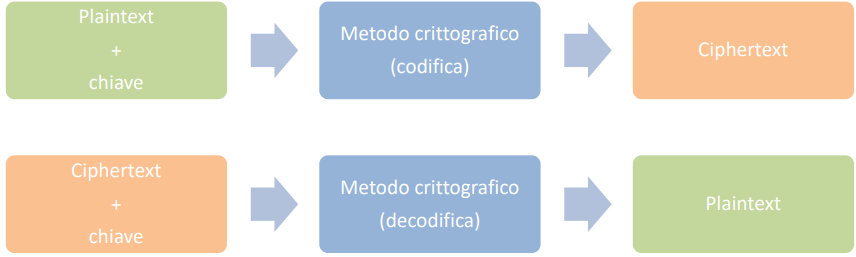
\includegraphics[width=5.42188in,height=0.57641in]{media/image19.png}

\begin{itemize}
\item
  Canali utilizzabili nel 2.5 Ghz
\end{itemize}

\begin{enumerate}
\def\labelenumi{\arabic{enumi}.}
\setcounter{enumi}{5}
\item
  IPv6 prevede indirizzi lunghi:

  \begin{itemize}
  \item
    \textbf{128 bit}
  \end{itemize}
\item
  Converti da Hex a binario:

  \begin{itemize}
  \item
    8: \textbf{1000}
  \item
    F: \textbf{1111}
  \item
    0: \textbf{0000}
  \end{itemize}
\item
  Abbrevia F520:7F6B:A03F:0000:0000:0053:0000:2DCF:

  \begin{itemize}
  \item
    \textbf{F520:7F6B:A03F::53:0:2DCF}
  \end{itemize}
\item
  Protocollo 802.1Q prevede al massimo quante VLAN:

  \begin{itemize}
  \item
    \textbf{4096}
  \end{itemize}
\item
  Scrivi il prefisso, non abbreviato, di 210F::AAAA:B080:7878:9009/64:

  \begin{itemize}
  \item
    \textbf{\emph{210F:0000:0000:0000}:0000:0000:0000:0000/64}
  \end{itemize}
\item
  Quali indirizzi IPv6 funzionano in modo simile a quelli privati IPV4:

  \begin{itemize}
  \item
    \textbf{Unique local}
  \end{itemize}
\item
  Metrica usata da OSPF per scegliere il percorso migliore:

  \begin{itemize}
  \item
    \textbf{Cost}
  \end{itemize}
\item
  Scrivi il subnet ID di 172.16.150.41/18:

  \begin{itemize}
  \item
    \textbf{172.16.128.0}
  \end{itemize}
\item
  Administrative distance di default per rotta statica è:

  \begin{itemize}
  \item
    1
  \end{itemize}
\item
  OSPF multiarea, caratteristiche di un Area Border Router:

  \begin{itemize}
  \item
    \textbf{Sta sia nella backbone sia nella singola area}
  \end{itemize}
\item
  Converti da decimale a binario:

  \begin{itemize}
  \item
    259: \textbf{100000011}
  \item
    111: \textbf{1101111}
  \item
  \end{itemize}
\item
  PortFast va attivato nelle porte destinate alla connessione con:

  \begin{itemize}
  \item
    \textbf{PC}
  \item
    \textbf{Notebook}
  \end{itemize}
\item
  Rota statica che mandi tutto il traffico destinato alla rete
  192.168.15.0/24 verso 182.168.2.6:

  \begin{itemize}
  \item
    \textbf{ip route 192.168.15.0 255.255.255.0 182.168.2.6}
  \end{itemize}
\item
\item
  Subnetting della rete 172.10.0.0/16 per consentire 800 host per
  sottorete:

  \begin{itemize}
  \item
    Classe:
  \item
    Nuova maschera
  \item
    Numero di sottoreti:
  \item
    Host per subnet:
  \item
    Subnet ID della prima sottorete:
  \item
    Broadcast address della prima sottorete:
  \end{itemize}
\item
  Quante reti IPv4 private di classe B esistono:

  \begin{itemize}
  \item
    \textbf{16}
  \end{itemize}
\item
  Classe dell'indirizzo 224.1.1.1:

  \begin{itemize}
  \item
    \textbf{D}
  \end{itemize}
\item
  L'utilizzo di due link paralleli tra SW1 e SW2, non bloccati da STP è
  possibile grazie a cosa:

  \begin{itemize}
  \item
    \textbf{PortFast}
  \end{itemize}
\item
  Se l'IP viene scelto dal Server tramite un pool e resta assegnato ad
  un certo MAC che tipo di DHCP è:

  \begin{itemize}
  \item
    \textbf{Automatico}
  \end{itemize}
\item
  Comando per abilitare Telnet in aggiunta a SSH:

  \begin{itemize}
  \item
    \textbf{transport input telnet ssh}
  \end{itemize}
\item
  Quale modalità di VTP non è possibile creare VLAN:

  \begin{itemize}
  \item
    \textbf{VTP client mode}
  \end{itemize}
\item
  Sinonimo di layer 3:

  \begin{itemize}
  \item
    \textbf{Livello di rete}
  \end{itemize}
\item
  Il comando \emph{interface gigabitethernet 0/0 20} crea cosa:

  \begin{itemize}
  \item
    \textbf{VLAN}
  \end{itemize}
\item
  Quale tra questo è un indirizzo IPv6 unique local:

  \begin{itemize}
  \item
    \textbf{\emph{FD}6D:8D64:AF0C:2::}
  \end{itemize}
\item
  Quale OSPF neighbor state è atteso quando lo scambio di informazioni
  sulla topologia è in corso:

  \begin{itemize}
  \item
    \textbf{2-way}
  \end{itemize}
\item
  I router non instradano i pacchetti di che tipo:

  \begin{itemize}
  \item
    \textbf{Link local}
  \end{itemize}
\item
  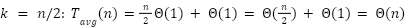
\includegraphics[width=4.92188in,height=1.92133in]{media/image77.png}

  \begin{itemize}
  \item
    \textbf{Configurando RootGuard su Switch C}
  \end{itemize}
\item
  Come si può ottimizzare il processo di manutenere e configurare
  innumerevoli VLAN:

  \begin{itemize}
  \item
    \textbf{Usando VTP}
  \end{itemize}
\item
  Con quale soluzione posso rimuovere uno dei due link tra switch:
\end{enumerate}

\begin{quote}
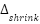
\includegraphics[width=2.19792in,height=1.34375in]{media/image98.png}
\end{quote}

\begin{itemize}
\item
  \textbf{Trunking}
\end{itemize}

\begin{enumerate}
\def\labelenumi{\arabic{enumi}.}
\setcounter{enumi}{34}
\item
  Scrivi accanto a ogni concetto il livello della pila TCP/IP a cui
  appartiene:

  \begin{itemize}
  \item
    Richiesta HTTP: \textbf{Layer 5}
  \item
    Default gateway: \textbf{Layer 3}
  \end{itemize}
\item
  NTP sta per:

  \begin{itemize}
  \item
    \textbf{Network Time Protocol}
  \end{itemize}
\item
  Sinonimo per layer 4:

  \begin{itemize}
  \item
    \textbf{Transport}
  \end{itemize}
\item
  A cosa può servire configurare una sottointerfaccia:

  \begin{itemize}
  \item
    \textbf{Configurare il trunking o ROAS}
  \end{itemize}
\item
  Quale tra queste non è una fase del lavoro di OSPF

  \begin{itemize}
  \item
    \textbf{Counting hops}
  \end{itemize}
\item
  Cos'è il roaming:

  \begin{itemize}
  \item
    \textbf{Passaggio da una cella ad un'altra}
  \end{itemize}
\item
  Quale bridge IP vince le elezioni STP come root:

  \begin{itemize}
  \item
    \textbf{40097:0200:1000:1000}
  \end{itemize}
\item
  Host A è connesso alla VLAN 1 di SW1. Chi tipicamente ha un IP nella
  stessa subnet di A:

  \begin{itemize}
  \item
    \textbf{interface vlan 1 dello switch}
  \end{itemize}
\item
  Il messaggio layer 2 è detto:

  \begin{itemize}
  \item
    \textbf{frame}
  \end{itemize}
\item
\end{enumerate}

Networking

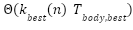
\includegraphics[width=6.26772in,height=1.59722in]{media/image59.png}

Con il termine \textbf{networking model} si riferisce ad un insieme di
documenti, ognuno dei quali descrive un aspetto di una rete.

Un documento può descrivere un protocollo (insieme di regole logiche che
i dispositivi devono seguire per comunicare) o requisiti fisici.

\section{TCP/IP}\label{tcpip}

Il modello supportato da tutti è \textbf{TCP/IP} che include una serie
di protocolli per far comunicare tra loro i computer, i protocolli
vengono definiti tramite i \textbf{Requests For Comments} (RFC).

TCP/IP include anche protocolli più vecchi non definiti tramite RFC,
come l'ethernet LAN, ma dal IEEE.

TCP/IP usa un modello a strati per rendere più comprensibile i network
model:

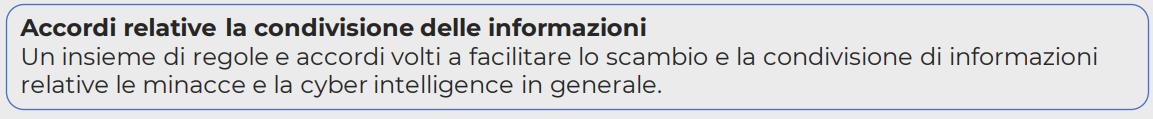
\includegraphics[width=1.71012in,height=2.52411in]{media/image88.png}

Il layer più basso si occupa della trasmissione dei bit su ogni canale
fisico, il data link su una tipologia di link fisico (ethernet o
wireless), il network si occupa della consegna dei dati attraverso
l'intero percorso e i due superiori riguardano le applicazioni che
ricevono/inviano i dati.

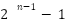
\includegraphics[width=6.26772in,height=1.43056in]{media/image10.png}

\subsection{Application layer}\label{application-layer}

I protocolli di questo livello forniscono servizi al software, NON
definisce l\textquotesingle applicazione ma i servizi da essa usati.

Es: un applicativo browser usa il protocollo HTTP.

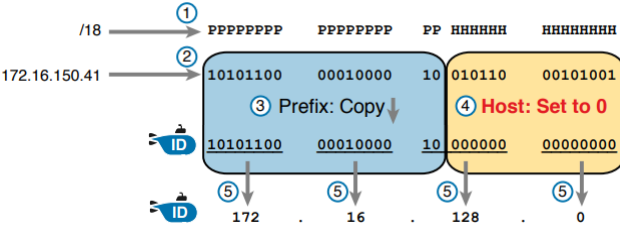
\includegraphics[width=6.26772in,height=1.81944in]{media/image103.png}

Notiamo come il terzo msg non ha un header perché il protocollo dopo il
primo messaggio li omette.

\subsection{Transport Layer}\label{transport-layer}

I protocolli di questo livello forniscono servizi a quelli superiori e
sono due:

\begin{itemize}
\item
  TCP: prima di inviare si assicura di instaurare una connessione, si
  occupa anche della correzione dei messaggi infatti ogni messaggio
  gestito dal TCP contiene un numero che indica il numero di sequenza di
  invio (SEQ), se il client riceve un numero che non corrisponde a
  quello che avrebbe dovuto ottenere (Es: 1-\textgreater2-\textgreater3
  ma ottiene 1-\textgreater3) capisce che uno è andato perso e richiede
  il rinvio.
\end{itemize}

\begin{quote}
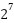
\includegraphics[width=4.26563in,height=1.33921in]{media/image11.png}
\end{quote}

\begin{itemize}
\item
  UDP: meno usato e non si ha la certezza dell'arrivo dei messaggi.
\end{itemize}

\subsubsection{Same/adjacent-layer
interaction}\label{sameadjacent-layer-interaction}

Il adjacent-layer interaction è quando livelli adiacenti (diversi)
lavorino insieme sullo stesso computer; es: HTTP usa il ripristino degli
errori di TCP.

Il same-layer interaction è quando due livelli uguali comunicano su due
computer diversi e quindi utilizzano i loro header per scambiarsi
messaggi; es: Larry e Bob usano i SEQ per controllare che i messaggi
siano arrivati nell'ordine giusto.

\subsection{Network layer}\label{network-layer}

In questo livello il protocollo principale è IP, fra le principali
funzionalità ci sono l'indirizzamento e l\textquotesingle instradamento.

Per funzionare IP definisce che ogni host deve avere un proprio
indirizzo univoco in maniera da essere identificato in una rete, è
composto da 4 numeri separati da punto (notazione dotted-decimal).

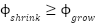
\includegraphics[width=5.00932in,height=2.13021in]{media/image107.png}

Altri protocolli di rete sono:

\begin{itemize}
\item
  \textbf{DNS}: serve per identificare i device grazie agli hostname.
\end{itemize}

\begin{quote}
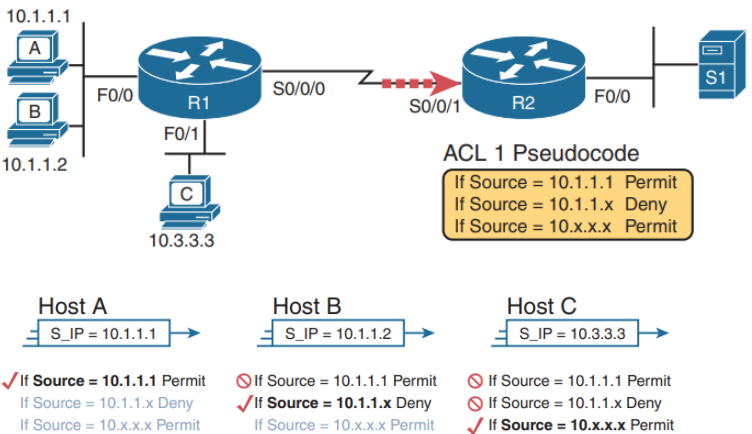
\includegraphics[width=5.0833in,height=1.64658in]{media/image163.png}
\end{quote}

\begin{itemize}
\item
  \textbf{ARP}: serve per apprendere dinamicamente l'indirizzo MAC di
  qualsiasi macchina connessa alla rete, per farlo il protocollo invia
  un messaggio in broadcast chiedendo di chi è il MAC da cercare.
\item
  \textbf{PING}: utilizza un altro protocollo chiamato ICMP, serve per
  testare la connessione fra due apparati.
\end{itemize}

\subsection{Data-Link e Physical
layer}\label{data-link-e-physical-layer}

Lavorano a stretto contatto per definire protocolli e tipo di hardware
necessari per recapitare dati attraverso una rete fisica.

Il physical si occupa di aspetti di cablaggio e segnali elettrici, ma
alcune convenzioni su questi argomenti spettano comunque al data-link.

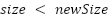
\includegraphics[width=4.88374in,height=1.74169in]{media/image93.png}

\section{Data encapsulation
terminology}\label{data-encapsulation-terminology}

Indica il processo di aggiungere header e trailer attorno ai dati
gestiti dai vari livelli.

Ogni livello aggiunge qualcosa al dato:

\begin{itemize}
\item
  \textbf{Application}: un msg HTTP può restituire un OK nel header;
\item
  \textbf{Transport}: il messaggio + header application viene processato
  dal transport che mette il proprio header TCP o UDP;
\item
  \textbf{Network}: come prima al nuovo messaggio aggiungiamo un altro
  header che contiene i vari indirizzi IP;
\item
  \textbf{Data-Link}: il data link aggiunge non solo un header ma anche
  un trailer finale
\item
  \textbf{Physical}: non aggiunge nulla e si occupa di inviare il
  messaggio.
\end{itemize}

Ogni messaggio cambia nome in base a che header ha al momento:

\begin{itemize}
\item
  \textbf{Data + TCP}: Segmento;
\item
  \textbf{Data + IP}: Pacchetto;
\item
  \textbf{Data + Data-Link trailer e header}: Frame.
\end{itemize}

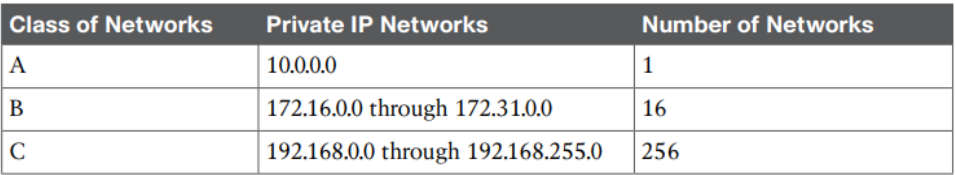
\includegraphics[width=6.26772in,height=4.08333in]{media/image45.png}

Oltre ai nomi detti sopra ogni PDU (il messaggio + header/trailer) può
essere identificato con il numero del livello, es: \textbf{Data +
Data-Link} = L2PDU (perchè livello 2).

\section{Ethernet LAN}\label{ethernet-lan}

Lo standard ethernet non è solo rame, comprende diverse tipologie di
cavi.

Noi vedremo lo standard applicato ad una LAN SOHO(small office/home
office), per creare una LAN si necessita di un device detto Ethernet LAN
switch, che ha porte dove connettere i cavi (necessariamente conformi
allo standard ethernet).

Nelle SOHO si usa un altro standard che è il wireless che può essere
utilizzato insieme all'ethernet per fornire connessioni cablate e non,
per utilizzare il wireless ci viene in aiuto l'access point (AP) che
agisce come uno switch ma per i device senza cavi.

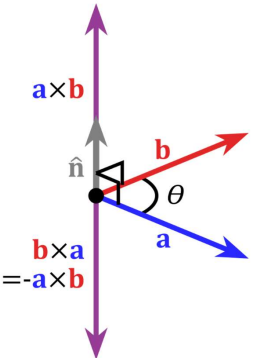
\includegraphics[width=4.45313in,height=1.30931in]{media/image76.png}

Quello appena detto è valido per le reti SOHO ma per quelle aziendali le
esigenze sono maggiori.

Prendendo come esempio un edificio a tre piani ogni piano dovrà avere
uno switch LAN ethernet e un AP LAN wireless, per comunicare fra piano a
piano si utilizza un altro switch che farà da collegamento fra i vari
switch di piano e il router per uscire dalla rete.

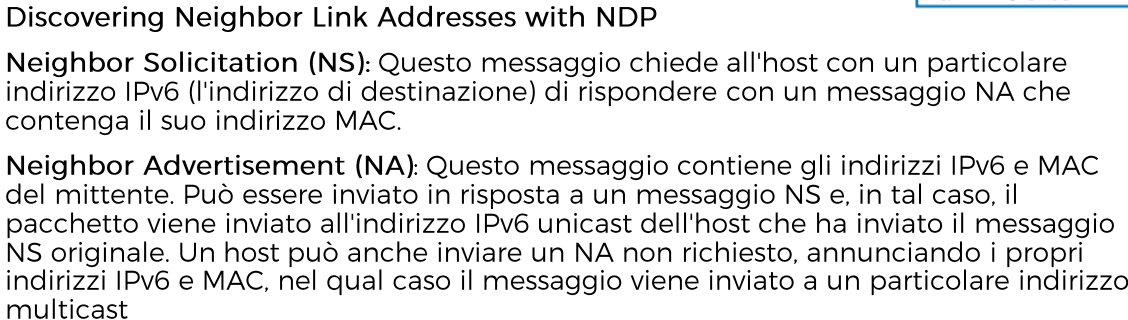
\includegraphics[width=4.80079in,height=2.43229in]{media/image112.png}

\subsection{Standard Ethernet nel physical
layer}\label{standard-ethernet-nel-physical-layer}

Come detto precedentemente l'Ethernet si riferisce a vari standard,
eccone alcuni:

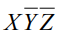
\includegraphics[width=6.26772in,height=1.875in]{media/image52.png}

Tutti questi standard possono essere utilizzati anche insieme nella
stessa rete nonostante le diverse velocità, questo perché Ethernet
agisce come singola tecnologia visto che utilizza lo stesso standard a
livello data-link.

\subsection{Cavi}\label{cavi}

\subsubsection{UTP - Twisted Pairs}\label{utp---twisted-pairs}

Sono composti da 2 o 4 coppie di fili in rame intrecciate su se stesse,
le coppie rappresentano un circuito elettrico chiuso e come connettore
si usa RJ45.

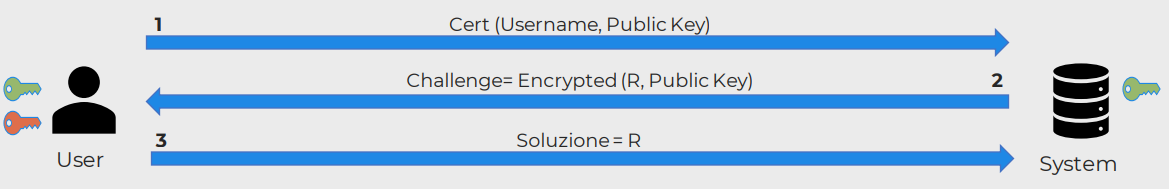
\includegraphics[width=4.16146in,height=1.20973in]{media/image111.png}

Gli standard 10BASE-T/100BASE-T utilizzano due coppie di fili in ogni
cavo per ciascuna direzione, i \textbf{trasmettitori} delle Network
Interface Card (NIC) utilizzano la coppia collegata ai pin \textbf{1,2}
i \textbf{ricevitori} quella ai pin \textbf{3,6}. \emph{Gli switch fanno
l'opposto}.

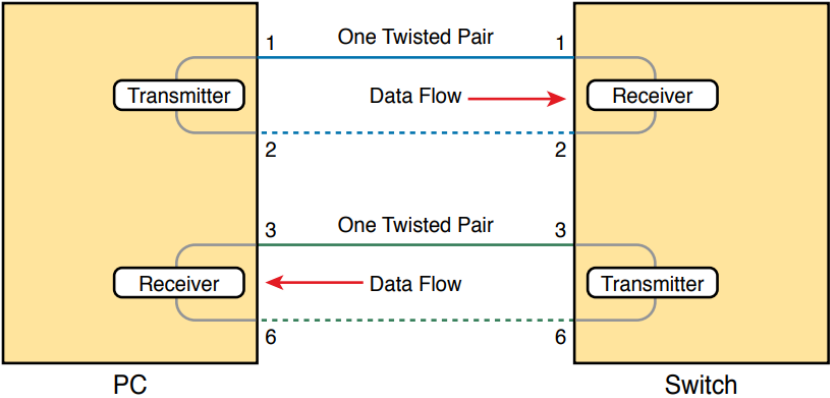
\includegraphics[width=4.8026in,height=2.45313in]{media/image160.png}

Un cavo straight-through funziona solo solo se i nodi utilizzano coppie
opposte, quindi se provo a connettere due dispositivi simili con questo
cavo la comunicazione non può avvenire perché usano gli stessi pin per
ricevere/trasmettere, per questo è nato il \textbf{crossover}.

Gli switch Cisco hanno la possibilità di cambiare alcune porte dopo
l'acquisto, come:

\begin{itemize}
\item
  Gigabit Ethernet Interface Converter (GBIC): rimuovibile per
  interfacce gigabit;
\item
  Small Form Pluggable (SFP): messo al posto del GBIC;
\item
  Small Form Pluggable Plus (SFP+): come l'SFP ma utilizza interfacce da
  10 Gbps.
\end{itemize}

\subsubsection{Fiber Cabling}\label{fiber-cabling}

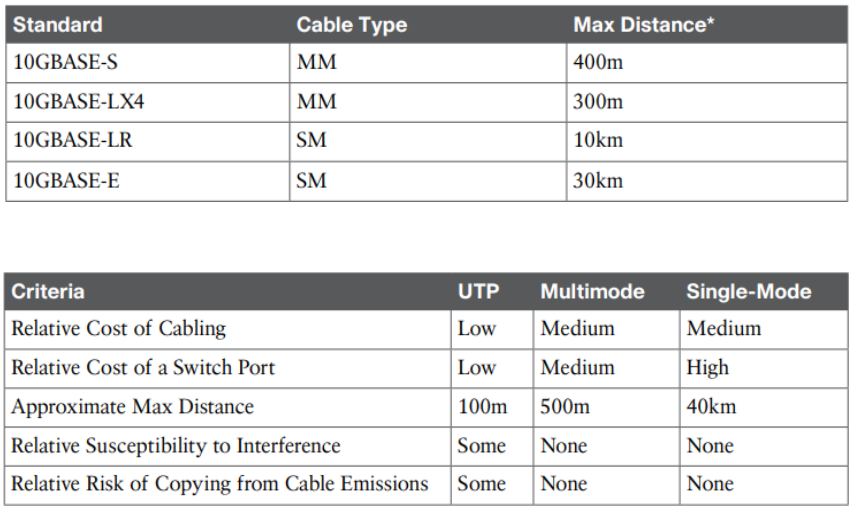
\includegraphics[width=3.7603in,height=2.09877in]{media/image153.png}

Il cavo può essere multimodale, cioè il core permettere più angoli di
trasmissione della luce e il segnale viene generato da un led:

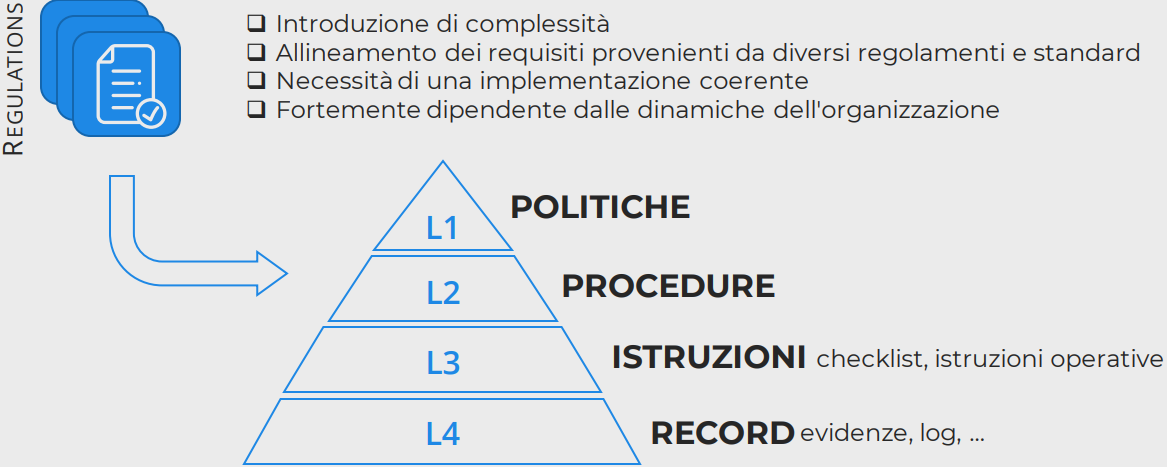
\includegraphics[width=6.26772in,height=1.45833in]{media/image18.png}

Oppure monomodale con un core più sottile (¼ del multimodale) e la
trasmissione avviene tramite laser:

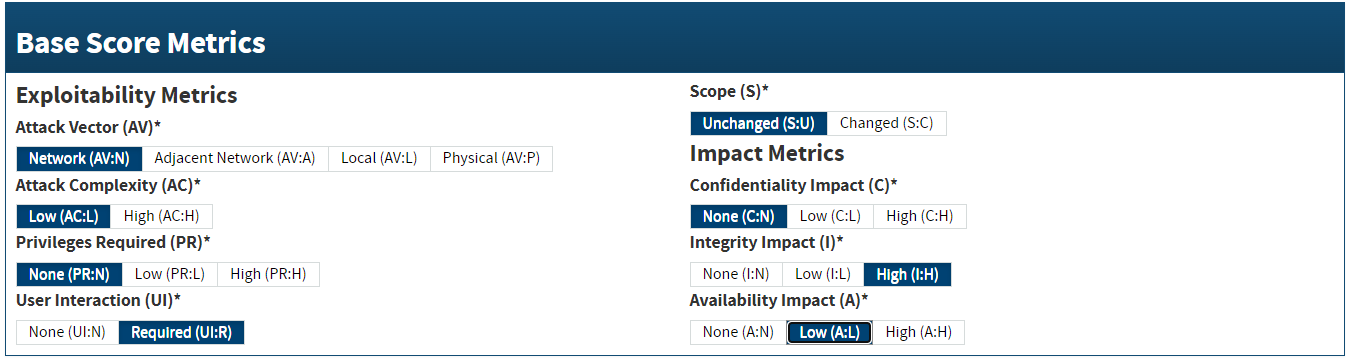
\includegraphics[width=6.26772in,height=1.40278in]{media/image26.png}

Prima di mostrare le caratteristiche va ricordato che è necessario avere
due cavi uno per direzione e la porta di trasmissione su un dispositivo
si collega a un cavo diretto verso una porta di ricezione sull'altro
dispositivo e viceversa.

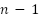
\includegraphics[width=6.26772in,height=3.75in]{media/image151.png}

\subsection{Frame Ethernet}\label{frame-ethernet}

Il frame ethernet è composto da diversi campi, vediamoli nel dettaglio:

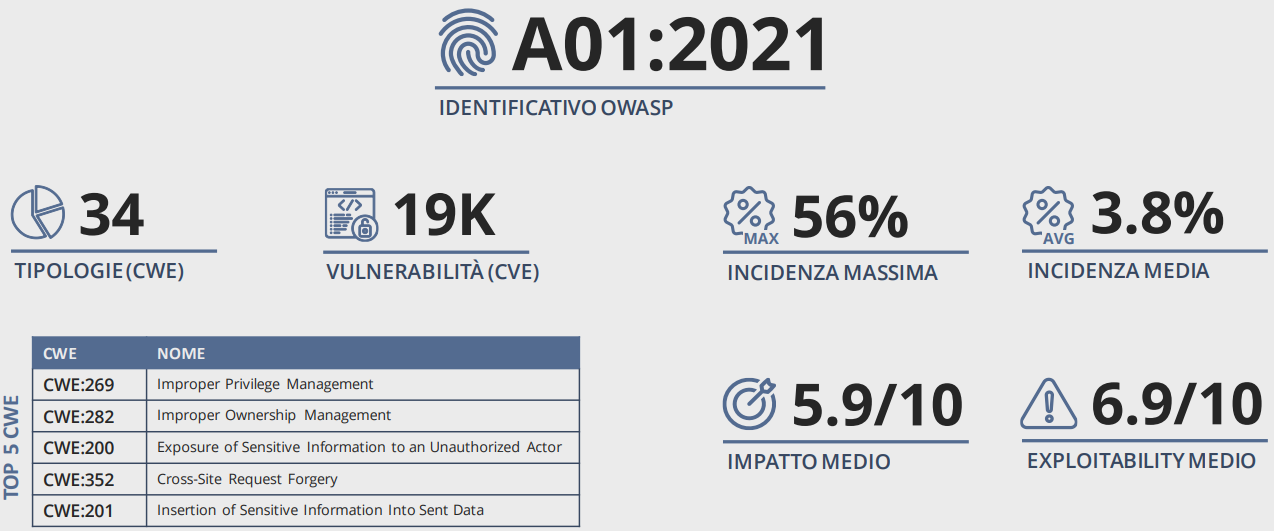
\includegraphics[width=6.26772in,height=4.5in]{media/image85.png}

Il MAC è un indirizzo formato da numeri binari (6 byte/48 bit) che
identificano in maniera univoca e universale un apparato di rete.

Vengono scritti anche in esadecimale con 12 cifre divisi da punti per
comodità (es: 0000.0C12.3456), dove i primi 3 byte identificano il
produttore ed è detto OUI rilasciato dal IEEE ed è univoco, gli altri 3
sono creati dal produttore e anch'essi sono univoci ma solo per i
prodotti dello stesso produttore.

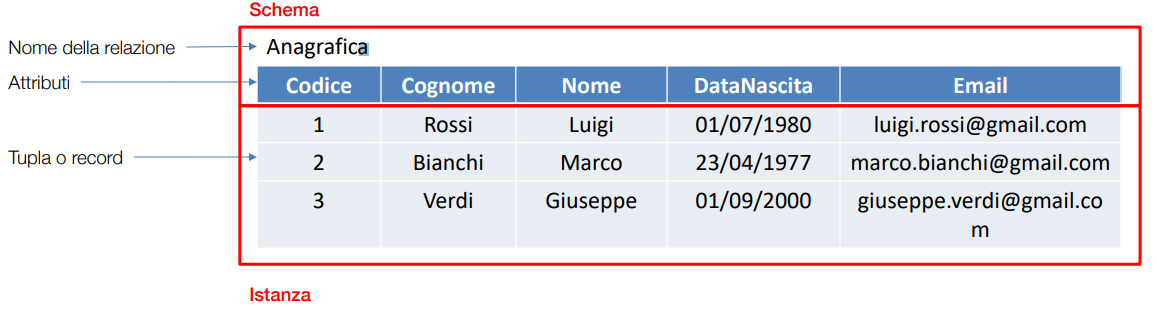
\includegraphics[width=4.97597in,height=1.65315in]{media/image69.png}

Va puntualizzato che il \textbf{FCS} controlla solo se sono avvenuti
errori per decidere se scartare o meno il frame, quindi non si occupa
della correzione dell'errore.

Per funzionare il mittente applica una formula matematica nota al frame
e mette il risultato dentro al campo frame, il ricevitore applica la
stessa formula al frame e controlla il risultato con il campo FCS.

\section{WAN}\label{wan}

Più LAN distanti fra loro collegate formano una WAN, il primo tipo è la
\textbf{Leased-Line} \textbf{WANs}, fornita da un provider e pagata
tramite abbonamento, da parte del cliente sembra di lavorare come una
normalissima connessione con cavo Ethernet ma in realtà può essere
composta da un alto numero di device.

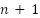
\includegraphics[width=6.26772in,height=3.29167in]{media/image158.png}

La leased offre un servizio a layer 1, dove recapita i bit tra
dispositivi collegati alla leased line stessa senza protocolli
data-link.

Successivamente si è iniziato a offrire protocolli per il livello
data-link tra cui \textbf{High-Level Data Link} (HDLC) e
\textbf{Point-to-Point} (PPP).

\subsection{\texorpdfstring{\protect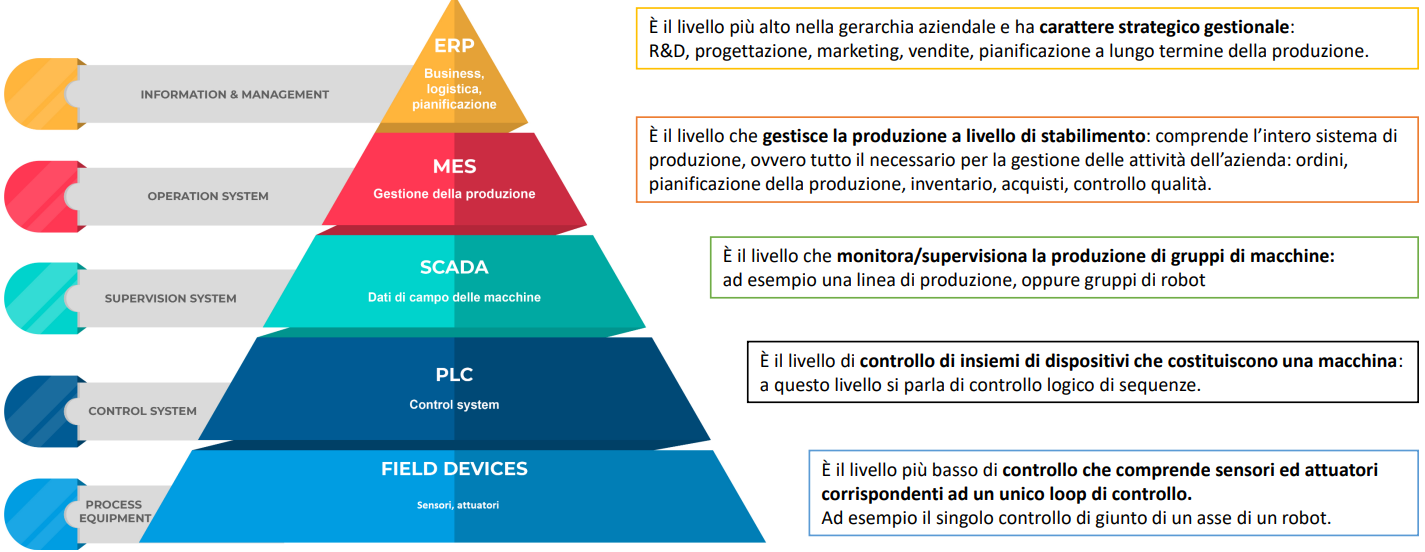
\includegraphics[width=6.26772in,height=3.27778in]{media/image123.png}}{}}\label{section}

\subsection{Ethernet WAN}\label{ethernet-wan}

IEEE ha migliorato l\textquotesingle Ethernet per renderlo compatibile
con la metodologia WAN. Per connettersi il cliente utilizza il router
che tramite un collegamento in fibra lascia l\textquotesingle edificio
per collegarsi al service provider tramite un PoP (point of presence)
che normalmente è uno switch. Da questo punto il provider può utilizzare
qualsiasi tecnologia per creare servizi WAN.

Logicamente è una connessione point-to-point fisicamente è come una
connessione in fibra tra router.

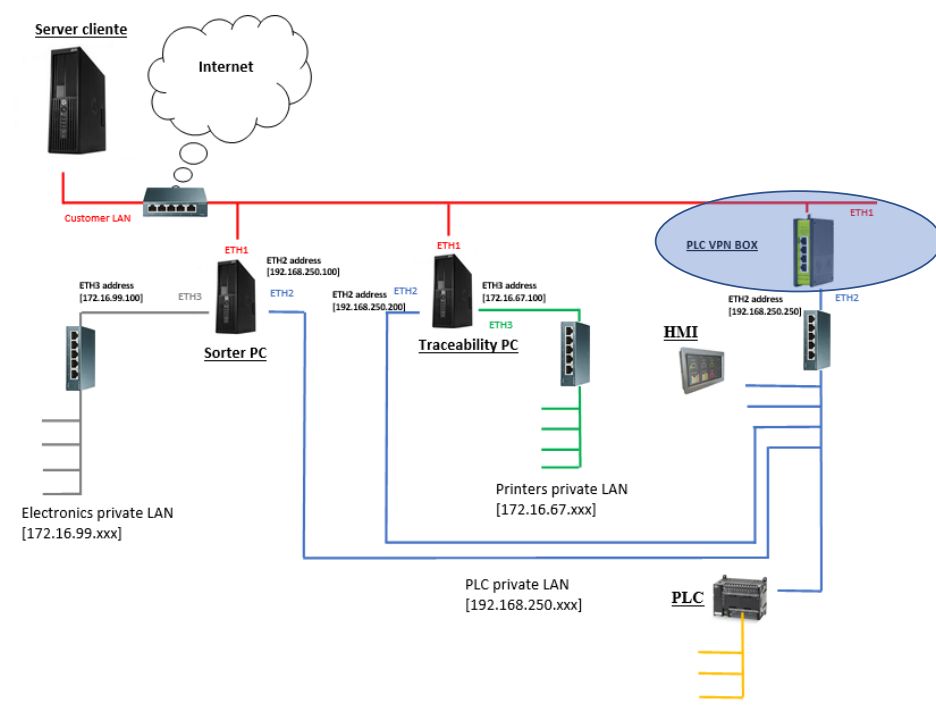
\includegraphics[width=6.26772in,height=2.08333in]{media/image136.png}

Una tecnologia utilizzata dal provider tra i due router è la EoMPLS, un
termine che si riferisce al Multiprotocol Label Switching, una
tecnologia che viene usata per creare il servizio Ethernet per il
cliente.

Il collegamento utilizza gli stessi header/trailer Ethernet usati per la
LAN.

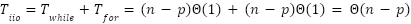
\includegraphics[width=6.26772in,height=2.02778in]{media/image159.png}

\section{IP Routing}\label{ip-routing}

L'IP si occupa dei dettagli logici della consegna dei dati, nel
dettaglio come i pacchetti viaggiano end-to-end su una rete TCP/IP anche
passando attraverso LAN e WAN.

Per rendere possibile questo i router e pc lavorano insieme per eseguire
il routing, infatti il PC ha un software che dice dove inviare i
pacchetti, di solito al router più vicino e da lì in poi il router
sceglie a chi inviarlo.

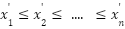
\includegraphics[width=4.43715in,height=3.69271in]{media/image148.png}

In questo esempio il PC1 nota che l'ind ip del PC2 non è nella sua
sottorete per questo invia il messaggio a qualcuno con il compito
dell'instradamento, il router della sua LAN.

Il router è in grado di instradare correttamente il pacchetto perchè al
suo interno tiene traccia di tutti gli indirizzi ip delle reti con cui
può comunicare e come raggiungerle, salva tutto nella tabella di
routing.

Ora vediamo i passaggi uno dopo l'altro con anche i vari incapsulamenti
effettuati dai protocolli utilizzati:

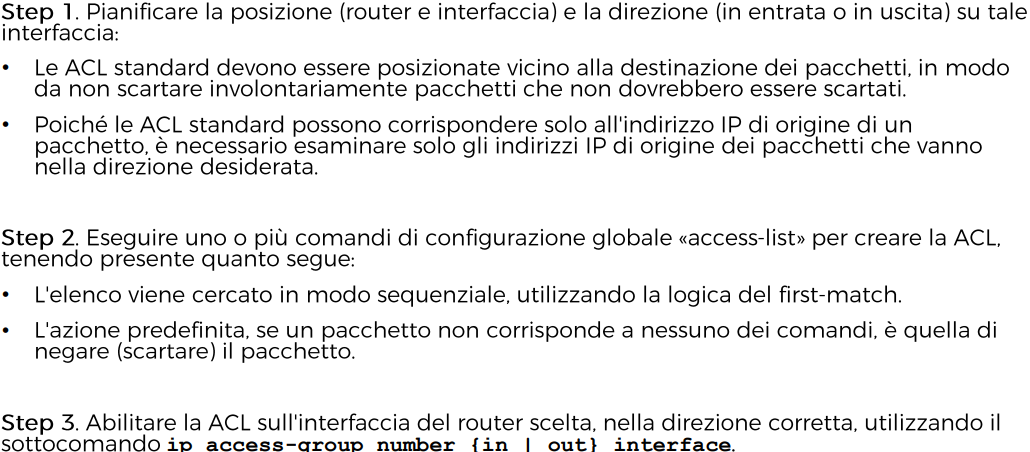
\includegraphics[width=7.00132in,height=2.82611in]{media/image117.png}

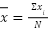
\includegraphics[width=6.94362in,height=2.84896in]{media/image54.png}

L'header IP è così formato:

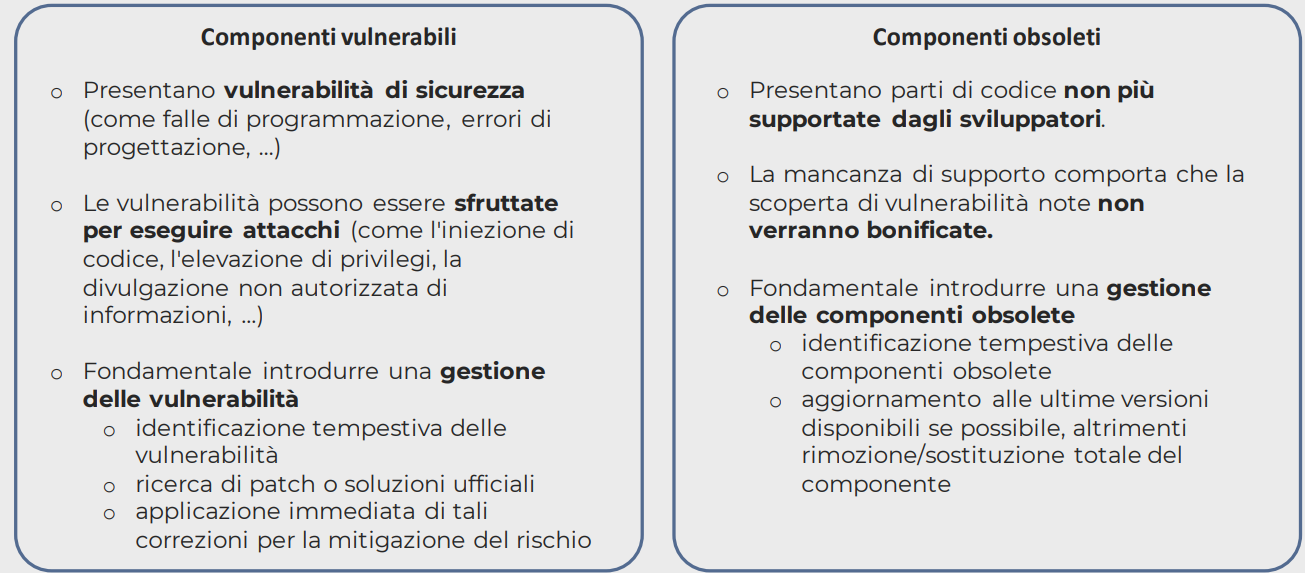
\includegraphics[width=6.26772in,height=2.02778in]{media/image116.png}

CLI

Possiamo collegarci ad uno switch per configurarlo tramite ssh o cavo.

Se il collegamento è via cavo usiamo un cavo azzurro detto cavo console

\subsection{AAA}\label{aaa}

Se in una azienda sono presenti innumerevoli device con utenti replicati
su ognuno, è possibile adottare un server per l'autenticazione.

\emph{``Authentication, authorization, and accounting (AAA) server''}

Questo server ospita username e password in modo centralizzato. Quando
un AAA server è configurato, lo switch invia un messaggio contenente
username e password al server stesso, il quale risponde comunicando se
l'accesso è autorizzato.

I più conosciuti sono RADIUS e TACACS+

LAN SWITCHING

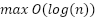
\includegraphics[width=6.26772in,height=4.56944in]{media/image149.png}

Le LAN permettono la comunicazione al loro interno e ad altre LAN
tramite switch che sanno a chi inviare i messaggi tramite MAC Address.

\emph{\textbf{Def}: tutti i device che si trovano sullo stesso broadcast
domain}

Il pacchetto che viene inviato dagli switch è di livello physical, ed è
così strutturato:

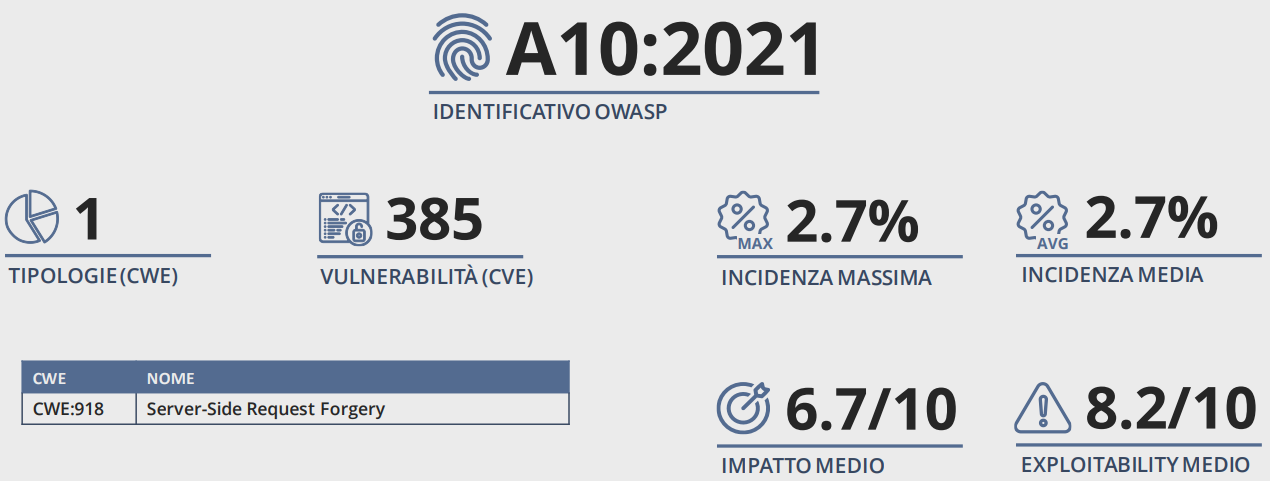
\includegraphics[width=4.53608in,height=3.31771in]{media/image70.png}

La porta verso la quale inoltrare il frame viene individuata grazie ad
una MAC address table, chiamata anche switching table. Questa tabella
riporta una lista di indirizzi e la relativa porta da utilizzare per
raggiungerli. Viene salvata in RAM e i record vengono salvati per 300
secondi.

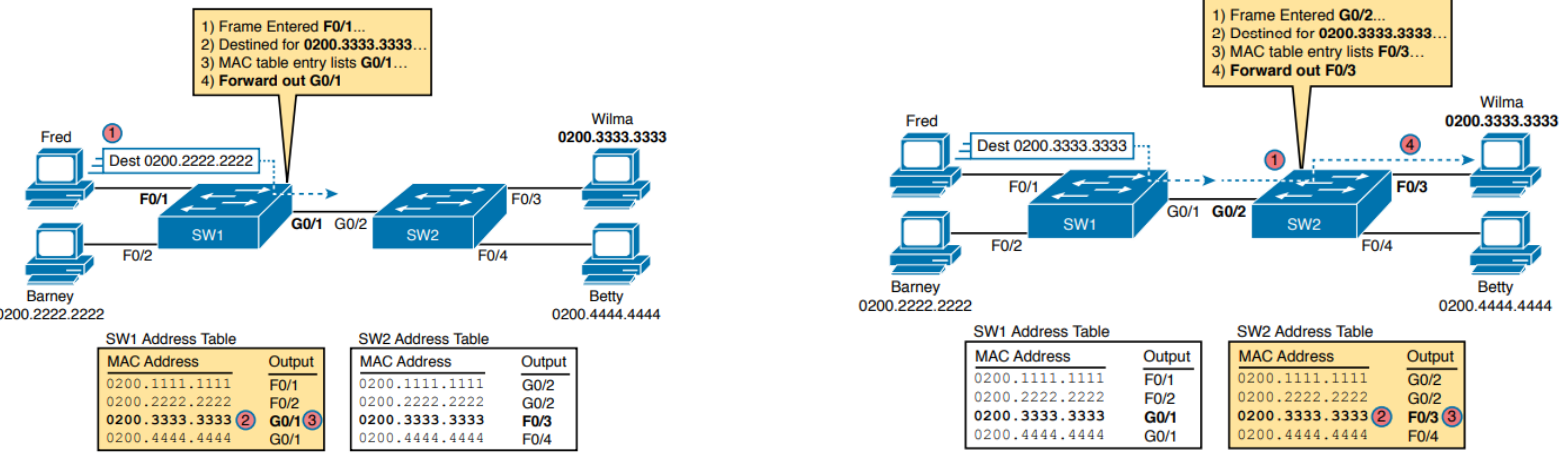
\includegraphics[width=6.26772in,height=1.83333in]{media/image63.png}

La costruzione della tabella avviene esaminando i source address dei
frame che entrano nella varie porte (chi invia popola NON chi lo
riceve).

Se un indirizzo non è presente nella tabella, una copia del frame viene
inoltrata verso ogni porta dello switch (ad eccezione di quella dalla
quale il frame è stato ricevuto). Questo processo si chiama flooding.

In questo modo il destinatario riceverà il messaggio e lo switch
imparerà la corretta porta per raggiungere quel MAC nel momento in cui
il destinatario invierà la risposta.

Usando il flooding può avvenire il problema del LOOP, dove il messaggio
gira all'infinito saturando la rete perchè la rete ha dei link
ridondanti.

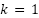
\includegraphics[width=4.05364in,height=1.38213in]{media/image165.png}

Per risolvere si usa il protocollo STP, dove alcuni link impediscono di
rinviare i messaggi rendendo possibile solo un path per collegare due
PC, nell'esempio sopra STP spegne Bob visto che Archie e Larry hanno
un'altro modo per comunicare.

\section{Switch interfaces}\label{switch-interfaces}

Se due switch in collegamento usano velocità differenti utilizzano un
meccanismo di auto-negoziazione per decidere una velocità consona per
entrambi, questo meccanismo funziona anche con i duplex (full, half,
auto).

La autonegoziazione è definita da uno standard IEEE, Cisco non lo
supporta perché le loro porte hanno un metodo loro per capire la
velocità, ecc.

Nel dettaglio i duplex:

\begin{itemize}
\item
  \textbf{Full}: entrambi i comunicanti ricevono e inviano
  contemporaneamente.
\item
  \textbf{Half}: in questo caso solo uno alla volta può trasmettere
  mentre l'altro ascolta. Viene usata dal Wi-Fi.
\end{itemize}

Per capire se un'interfaccia è collegata a qualcosa lo switch invia
degli impulsi detti LIT o Normal Link Pulses (NLP); successivamente sono
nati gli Fast Link Pulse.

Lo switch nella auto-negoziazione per capire la velocità usa il tipo di
impulso che gli arriva fra NLP o FLP.

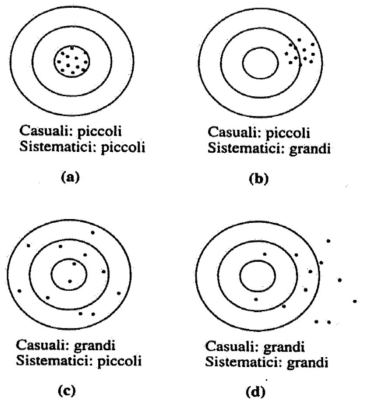
\includegraphics[width=6.26772in,height=2.61111in]{media/image80.png}

\section{STP}\label{stp}

\emph{Nella terminologia STP: switch \textless=\textgreater{} bridge}

Spanning Tree Protocol, protocollo per evitare che alcune porte
propaghino frame in maniera indefinita e duplicando i pacchetti.

Il problema sussiste se ci sono più path per unire gli stessi device,
per questo STP blocca le porte che non sono gli unici collegamenti con
una parte della rete.

I problemi causati dai frame in loop sono:

\begin{itemize}
\item
  \textbf{Broadcast storm}: in questo caso i link risultano saturi
  andando a perdere i veri pacchetti a causa di troppi frame broadcast o
  simili;
\item
  \textbf{MAC table instability}: in questa casistica le tabelle di
  indirizzi MAC cambiano in maniera incontrollata per via di frame con
  stesso source address MAC che gira e viene ricevuto su porte diverse.
\item
  \textbf{Multiple copies}: semplicemente lo stesso end device ottiene
  lo stesso pacchetto più volte duplicato, andando a rompere
  applicativi.
\end{itemize}

Ogni volta che colleghiamo un'interfaccia la verifichiamo prima che
possa inviare qualsiasi pacchetto, e la mettiamo in modalità
\emph{forwarding}, operano normalmente, o \emph{blocking},
\textbf{processano solo frame STP/RSTP}, (la modalità non influenza
altre info della porta come il trunking).

Esistono altre due modalità (non stabili) con cui lo switch può
impostare la porta, queste vengono usate durante il cambio da blocking a
forwarding, e sono:

\begin{itemize}
\item
  \textbf{listening}: si comporta come in blocking ma durante il periodo
  in cui è in questa modalità lo switch cancella dalla tabella MAC le
  voci per le quali non vengono ricevuti frame;
\item
  \textbf{learning}: si comporta come il blocking ma intanto ri-inizia a
  ripopolare la tabella con quello che riceve.
\end{itemize}

STP elegge uno switch root o root bridge con tutte le porte in
forwarding, tutti gli altri switch della rete devono attivare una porta
con cammino minimo (root port) per arrivare al root bridge e metterla in
forwarding.

Successivamente ogni switch rende la porta con root cost (costo per
arrivare al root bridge) più basso la \textbf{root port} (in
forwarding).

Con due switch collegati quello con root cost minore diventerà il
\textbf{designated switch} con la \textbf{designated port} connessa con
l'altro switch e andando a chiudere le altre.

Ogni switch ha un bridge ID (BID) da 8 byte ( 2 di priorità e 6 di ID)
univoco, per scambiarsi gli BID dei vicini si usano messaggi STP detti
BPDU, così composto:

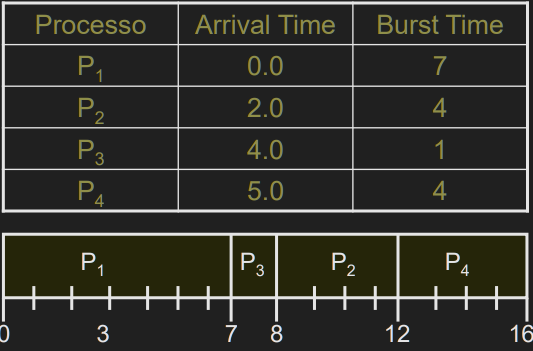
\includegraphics[width=6.26772in,height=1.81944in]{media/image48.png}

Il root bridge detto prima viene definito con il BID più basso, con BID
uguali si prende il MAC più basso (contenuto nel BID nella parte ID).

Uno switch smette di inviare BPDU con il proprio BID se riceve un BID
migliore da un altro perché capisce che non è lui il switch root.

\emph{Il root cost detto prima viene riportato in ogni BPDU ricevuto
sulla stessa interfaccia, il costo è un numero associato ad una
interfaccia.}

\emph{Se il root cost è uguale esistono 3 regole per scegliere il
percorso:}

\begin{enumerate}
\def\labelenumi{\arabic{enumi}.}
\item
  \emph{prendi il vicino con l'ID bridge migliore;}
\item
  \emph{scegli in base alla priorità della porta;}
\item
  \emph{scegli in base al numero di porta.}
\end{enumerate}

Sugli switch Cisco STP è attivo di default con un BID predefinito e le
interfacce hanno un costo predefinito basati sulla velocità. Tutto ciò è
comunque modificabile dal tecnico.

Riassumendo:

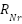
\includegraphics[width=6.26772in,height=2.05556in]{media/image53.png}

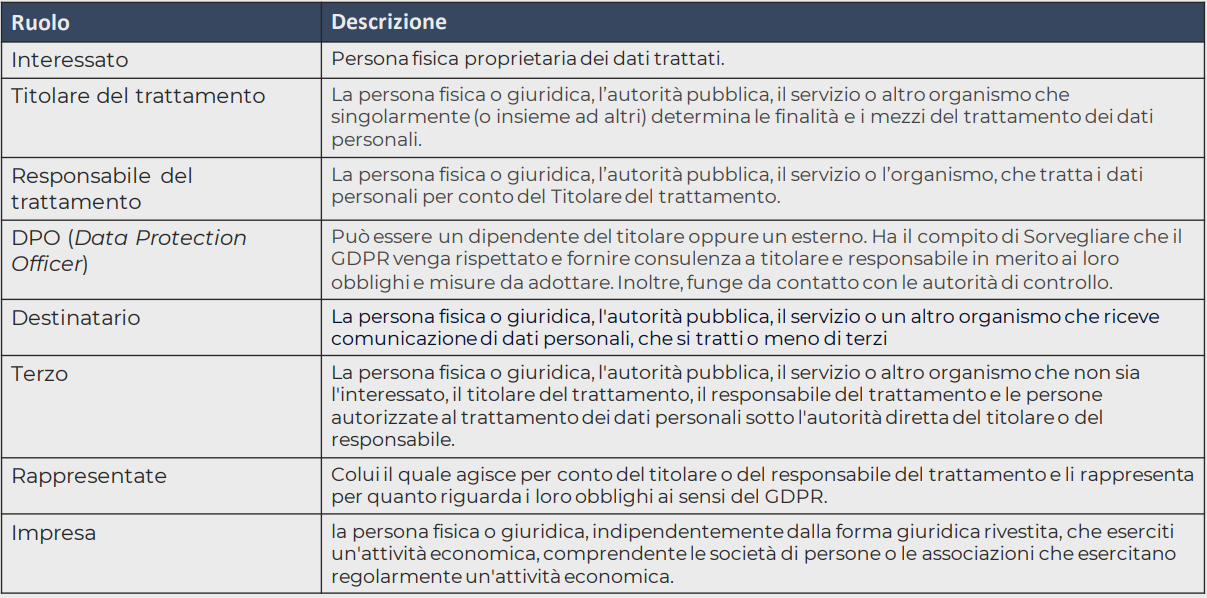
\includegraphics[width=3.48438in,height=2.81813in]{media/image110.png}

\subsubsection{RSTP}\label{rstp}

Il Rapid Spanning Tree Protocol è l'altra versione del protocollo che si
comporta normalmente tranne per alcune caratteristiche:

\begin{itemize}
\item
  è possibile che uno switch possa rimuovere la propria root port o
  sostituire la designated port senza attesa fra una modalità e l'altra
  (non sempre);
\item
  nuovi tipi di porte:
\end{itemize}

\begin{quote}
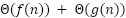
\includegraphics[width=4.51595in,height=1.23026in]{media/image46.png}

L'alternate è la seconda migliore scelta, andando a rimuovere i tempi di
attesa al cambio della root port.

La backup port si usa solo se sono presenti hub nelle reti.
\end{quote}

\begin{itemize}
\item
  gli switch generano i propri Hello (senza aspettare di riceverli) e
  possono fare query tra vicini.
\end{itemize}

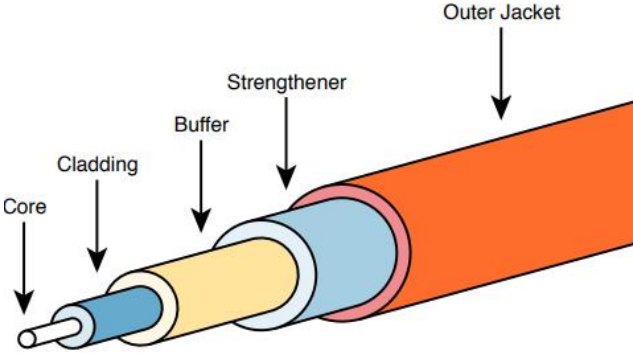
\includegraphics[width=6.26772in,height=2.94444in]{media/image150.png}

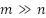
\includegraphics[width=6.26772in,height=1.33333in]{media/image141.png}

Le porte fra i due tipi di protocolli hanno stati uguali e diversi, a
volte cambiano i nomi:

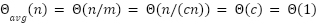
\includegraphics[width=5.60938in,height=1.86358in]{media/image137.png}

Per evitare la convergenza (cambiamento all'interno della rete), si
usano gli \textbf{EtherChannel} o PortChannel, quindi un canale con
diversi backup. STP tratta i cavi come uno unico nonostante fisicamente
c'è ne siano di più.

È possibile implementare il \textbf{PostFast} cioè al collegamento di un
end device alla rete saltiamo tutta la procedura STP, è molto pericoloso
per questo si usa solo con dispositivi che non provocano loop come PC o
laptop.

\subsubsection{Cisco STP}\label{cisco-stp}

Cisco ha creato protocolli paralleli ai due appena visto che funziona
sui propri dispositivi che da la possibilità di creare istanze spanning
tree per ogni VLAN:

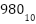
\includegraphics[width=6.26772in,height=1.91667in]{media/image32.png}

MSTP è come quelle di Cisco ma dell'IEEE.

Nelle versioni che supportano le VLAN il campi BID cambia:

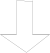
\includegraphics[width=6.26772in,height=2.25in]{media/image41.png}

\subsubsection{Root Guard}\label{root-guard}

Modalità che evita che un nuovo switch appena inserito in rete diventi
lo switch root. Può comunque stare connesso nella rete e utilizzare STP
o RSTP.

\subsubsection{BPDU Guard}\label{bpdu-guard}

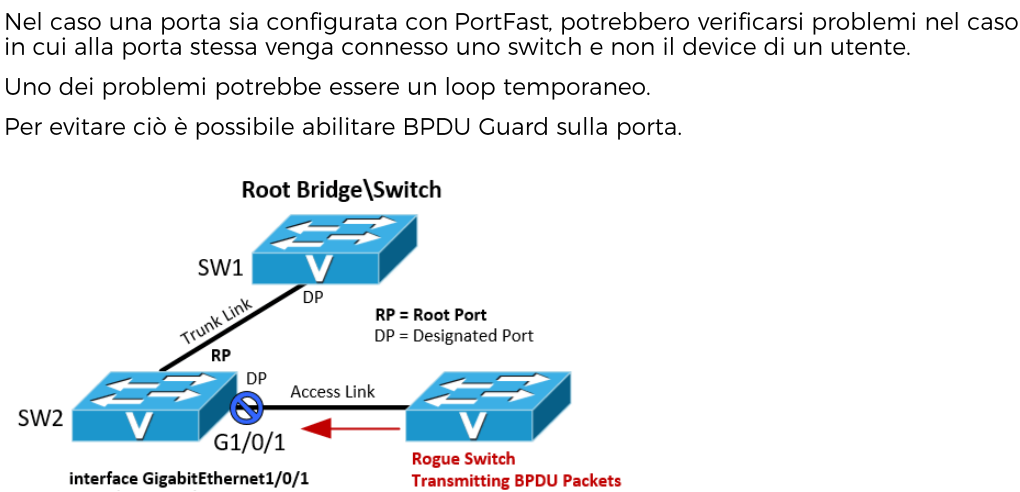
\includegraphics[width=6.26772in,height=3.02778in]{media/image15.png}

Praticamente spegne la porta quando nota che arrivano pacchetti tipici
di uno switch con STP, l'unico modo per riattivare la porta è farlo a
mano.

VLAN

Sono delle LAN virtuali quindi non fisicamente divisi da più switch, ma
più PC connessi allo stesso switch che però divide le proprie porte in
diverse LAN virtuali.

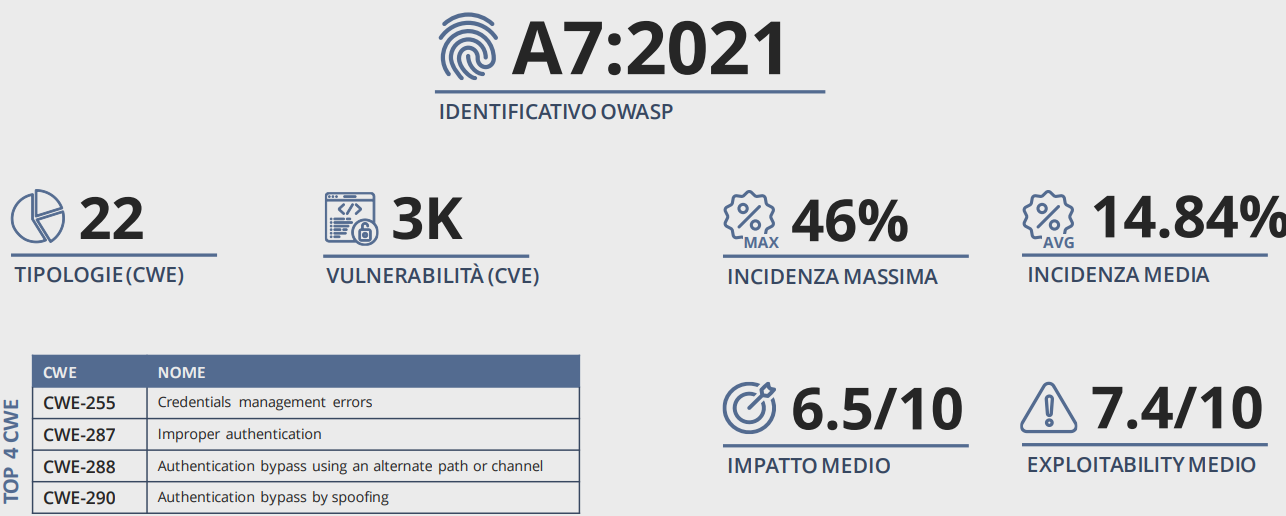
\includegraphics[width=6.26772in,height=0.95833in]{media/image94.png}

Le VLAN hanno diversi vantaggi:

\begin{itemize}
\item
  limitazione di device che ricevono messaggi inutili (messaggio
  broadcast);
\item
  riduzione dei problemi di sicurezza (se una vlan viene infettata le
  altre sono separate);
\item
  design di rete più flessibile.
\end{itemize}

\section{Trunking}\label{trunking}

Se ho più switch posso comunque usare le VLAN anche se non fisicamente
connessi allo stesso switch, questo è possibile dicendo che il link che
connette gli switch faccia parte della VLAN.

Per evitare di creare tot collegamenti fra switch per ogni VLAN usiamo
il \textbf{trunking}, quindi usiamo un unico collegamento tra switch a
switch dove facciamo passare le VLAN e per far capire verso quale VLAN
il frame è diretto lo \textbf{tagghiamo} (header con ID della VLAN).

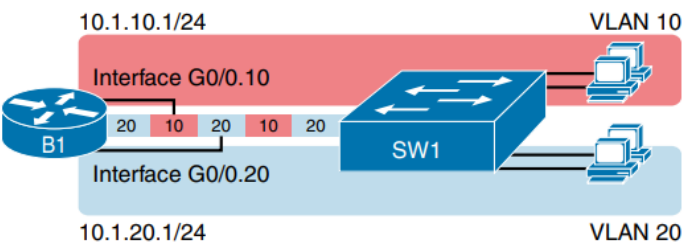
\includegraphics[width=6.26772in,height=3in]{media/image102.png}

Il protocollo di trunking è il IEEE 802.1Q (oppure Dot1q), che prevede 4
extra byte nell'header del frame ethernet.

12 di questi bit sono dedicati all'ID VLAN (possiamo gestire 4096 VLAN
possibili). Cisco divide il range da 1 a 1005 alla normal range e dal
1006 al 4095 al extended range.

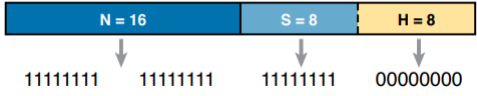
\includegraphics[width=5.05729in,height=1.60456in]{media/image122.png}

Il protocollo prevede una VLAN di default (di solito la 1 ma cambiabile)
che non viene taggata questo per far si di riuscire a comunicare con
dispositivi che non supportano il trunking; infatti tutti i frame non
taggati verranno indirizzati alla default.

\emph{\textbf{NON} è possibile che i messaggi riescano a passare da un
layer all'altro tramite switch quindi layer 2, l'unico modo è utilizzare
un router o uno switch multilayer che lavorano in layer 3.}

Nel trunking esistono diversi tipi di cavi uno in access e uno in trunk
più alcuni tipi dinamici

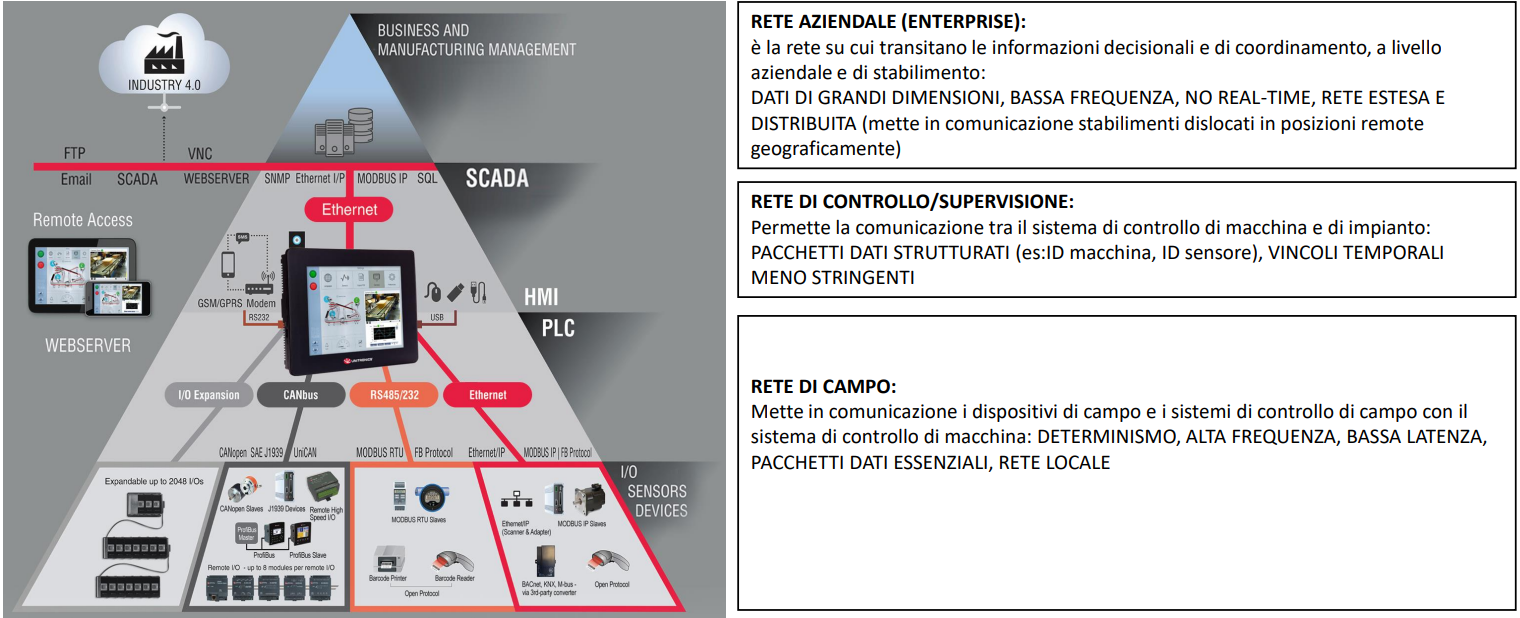
\includegraphics[width=6.26772in,height=0.84722in]{media/image40.png}

\subsection{VLAN Voice}\label{vlan-voice}

Cisco ha creato piccoli switch integrati nei telefoni fissi per ridurre
al minimo le connessioni tra PC e switch.

In questo modo i PC e i telefoni saranno in due VLAN separate con il
cavo che non può essere in access o in trunk e per questo esiste la
modalità voice.

\includegraphics[width=3.91146in,height=2.61227in]{media/image154.png}

Per attivare questa modalità il comando è:

\textbf{\hl{switchport voice vlan {[}num{]}}}

il resto dei comandi prima e dopo è uguale a quello per gestire le VLAN.

SUBNETTING

Una rete IP è una sequenza di indirizzi IP consecutivi che seguono una
regola nota, es: ind di rete 172.16.0.0, gli indirizzi saranno:
172.16.0.1-2-3-ecc.

Una subnet è un sottoinsieme di una rete di classe A,B o C.

Una subnet di classe B può essere 172.16.1 e un'altra con 172.16.2. Per
distinguere due sottoreti differenti oltre a vedere gli indirizzi IP
possiamo ricordarci che due subnet DEVONO essere separate da almeno un
router.

Ogni collegamento WAN (quello in rosso) per collegare ogni subnet è a
loro volta una subnet, con i propri indirizzi che verranno usati dal
router (i router avranno tanti indirizzi IP tante quante sono le subnet
a lui collegate).

\includegraphics[width=4.53667in,height=1.75126in]{media/image30.png}

Per capire come dividere la mia rete in subnet procediamo a step:

\begin{enumerate}
\def\labelenumi{\arabic{enumi}.}
\item
  Analisi esigenze:

  \begin{itemize}
  \item
    quali host devono essere raggruppati in subnet;
  \item
    quante subnet richiede la rete;
  \item
    quanti indirizzi IP richiede ciascuna subnet;
  \item
    tutte le subnet saranno grandi uguali?
  \end{itemize}
\end{enumerate}

\begin{quote}
Per sapere il numero di subnet necessarie può venire in aiuto il numero
di VLAN esistenti, infatti possiamo decidere di rendere ogni VLAN una
subnet. Vanno contati anche i collegamenti WAN.

\includegraphics[width=3.34091in,height=1.49286in]{media/image91.png}

Per esempio in questo esempio (contando che per ogni switch ci sia una
sola VLAN) saranno necessarie 7 subnet, 4 per ogni VLAN (switch) e uno
per ogni collegamento WAN o seriale.

Ora dobbiamo chiederci quanti host ci saranno e quindi quanti IP devo
riservare, un aiuto può arrivare contando quante persone dovranno
lavorare sulla rete più qualche server/stampante/ecc.

In conclusione decidiamo se dare ad ogni subnet la stessa dimensione o
meno, la dimensione è semplicemente il numero di indirizzi IP
utilizzabili. Normalmente si opta per avere tutte le subnet uguali per
evitare errori.

L\textquotesingle ingegnere incaricato della creazione delle subnet
assegna a ciascuna una \textbf{maschera di sottorete} (o subnet mask)
che definisce la dimensione della subnet associata. la subnet mask
identifica degli host bit, con lo scopo di identificare i diversi
indirizzi IP degli host nella subnet.

\emph{La subnet mask definisce} \(2^{H} - 2\) \emph{indirizzi usabili
dagli host, dove H sono gli host bit e i - 2 indirizzi sono riservati.}

I due riservati sono il numero di sottorete (il più basso, es: 10.0.0.0)
e l'ind. di broadcast (il più alto, es: 10.255.255.255).

Quindi i 32 bits di ogni indirizzo sono così divisi:

\includegraphics[width=3.12135in,height=1.13561in]{media/image47.png}

Per la subnet mask, dei 32 bit, lascio a 0 tutti i bit uguali agli host
bit e metto a 1 tutti gli altri:

\includegraphics[width=3.55729in,height=0.71593in]{media/image121.png}

Se ho deciso di voler fare ogni subnet grande uguale per decidere quanti
indirizzi riservare devo prendere la rete che avrà bisogno di più
indirizzi e trovare un H abbastanza grande che lo contenga. Se ho una
subnet che ha bisogno di 200 ind. allora avrò un H = 8
(\(2^{8} - 2\  = \ 254\)).

Se le subnet saranno diverse allora faremo lo stesso procedimento ma per
ogni subnet, in questo caso le maschere si chiamano VLSM
(variable-length subnet masks).
\end{quote}

\begin{enumerate}
\def\labelenumi{\arabic{enumi}.}
\setcounter{enumi}{1}
\item
  Design subnet:

  \begin{itemize}
  \item
    scegliere la rete;
  \item
    scegliere la maschera;
  \item
    elencare tutte le subnet.
  \end{itemize}
\item
  Plan implementation.
\end{enumerate}

\section{Esempio di progettazione}\label{esempio-di-progettazione}

\includegraphics[width=6.26772in,height=3.26389in]{media/image120.png}

\section{NAT}\label{nat}

Agli albori di internet ad ogni azienda che voleva usare il servizio gli
si dava un range di IP pubblici (es: tutti quelli con: 1.0.0.0) da
utilizzare per evitare duplicati.

Quando gli indirizzi iniziavano a diventare sempre di meno sono nate 3
soluzioni:

\begin{enumerate}
\def\labelenumi{\arabic{enumi}.}
\item
  nuova versione di IP (IPV6) con 128 bit per indirizzo;
\item
  invece di dare un\textquotesingle intera rete IP da ogno azienda gli
  diamo un solo sottoinsieme;
\item
  NAT protocollo per l'utilizzo di reti IP private.
\end{enumerate}

Il NAT è l'idea che ha preso più piede perché permette a più aziende di
utilizzare la stessa identica rete IP privata e per collegarsi
all'esterno si usa un indirizzo pubblico che non è solo di un'azienda ma
viene dato a diverse aziende in momenti diversi.

\section{Classi}\label{classi}

\includegraphics[width=6.26772in,height=1.69444in]{media/image84.png}

\includegraphics[width=5.87049in,height=2.14336in]{media/image132.png}

Gli indirizzi IP privati utilizzabili sono:

\includegraphics[width=5.93229in,height=1.09383in]{media/image31.png}

Ogni classe divide i propri indirizzi in due parti una per la rete e una
per gli host, i bit sono così divisi:

\includegraphics[width=3.6593in,height=1.56448in]{media/image74.png}

E l\textquotesingle ingegnere per creare le subnet prende in prestito
alcuni bit dalla parte degli host e li riserva per identificare le
subnet.

\includegraphics[width=6.26772in,height=2.65278in]{media/image67.png}

Esempio:

\includegraphics[width=6.26772in,height=1.94444in]{media/image162.png}

\subsection{Notazioni}\label{notazioni}

\subsubsection{DDN}\label{ddn}

La dotted-decimal notation converte ogni set di 8 bit in decimale,
esempio:

\emph{11111111 0000000 0000000 0000000 -\textgreater{} 255.0.0.0}

\includegraphics[width=2.98073in,height=2.85078in]{media/image133.png}

\subsubsection{Prefix}\label{prefix}

Si usa per identificare la maschera in forma compatta, sostanzialmente
si mette dopo l'indirizzo IP una barra (/) seguita dal numero di 1
presenti della subnet mask, esempio:

\emph{X.X.X.X/8 -\textgreater{} 11111111 0000000 0000000 0000000
-\textgreater{} 255.0.0.0}

\section{Riassunto}\label{riassunto}

\subsection{Subnet mask}\label{subnet-mask}

\includegraphics[width=6.26772in,height=2.20833in]{media/image89.png}

\subsection{Divisione ind.}\label{divisione-ind.}

\includegraphics[width=6.26772in,height=0.84722in]{media/image22.png}

\subsection{Ricerca ind. sottorete o ID di
sottorete}\label{ricerca-ind.-sottorete-o-id-di-sottorete}

\includegraphics[width=4.68229in,height=1.71114in]{media/image92.png}

Senza convertirlo in binario, se abbiamo la maschera scritta in
notazione DDN possiamo fare:

\includegraphics[width=5.63021in,height=1.04263in]{media/image66.png}

\includegraphics[width=5.41146in,height=2.52595in]{media/image60.png}

\subsection{Ricerca ind. broadcast}\label{ricerca-ind.-broadcast}

\includegraphics[width=4.86979in,height=1.58551in]{media/image144.png}

Senza convertirlo in binario, se abbiamo la maschera scritta in
notazione DDN possiamo fare:

\includegraphics[width=6.26772in,height=1.19444in]{media/image71.png}

\includegraphics[width=5.01563in,height=2.52547in]{media/image55.png}

ROUTING

Per connettere più LAN come già detto si usano le WAN se collocate in
maniera distante, per farlo si usano i router.

\section{Router}\label{router}

Ogni router ha delle porte gigabit ethernet (2 di solito), seriali e
almeno due slot vuoti dove inserire delle schede NIM, che permettono di
configurare il router come si vuole; e si possono spegnere e accendere a
piacimento (al contrario degli switch).

Switch e Router condividono molti comandi e caratteristiche riguardanti
la CLI, le differenze principali sono:

\begin{itemize}
\item
  conf ind. IP: ogni interfaccia può avere un ind. IP;
\item
  i router hanno una porta AUX per collegare modem e linee telefoniche
  per configurarli a distanza;
\item
  telnet e ssh disattivati di default (\emph{transport input none}, per
  attivarla).
\end{itemize}

\emph{I router iniziano a instradare pacchetti appena viene inserito un
indirizzo IP, se non è presente quella porta non riceve e non invia
messaggi.}

\section{IP routing}\label{ip-routing-1}

L'IP routing è il processo di instradamento di un pacchetto da un punto
A ad un punto B, utilizzando il layer 3.

L'host mittente crea un msg e lo invia al suo gateway predefinito, che a
sua volta tramite le proprie tabelle di routing sa dove instradarlo
correttamente.

\textbf{Nel dettaglio:}

\includegraphics[width=6.26772in,height=2.15278in]{media/image131.png}

Il router ha più lavori da fare rispetto all'host:

\begin{itemize}
\item
  elabora i frame data link, solo se non presenta errori (controlla il
  FCS, se capisce che ci sono stati errori lo scarta) e se l'ind. di
  destinazione data-link è il suo;
\item
  deincapsula il frame data-link, rimanendo con il pacchetto IP;
\item
  decide dove inviarlo, tramite confronto con routing table e ind. di
  destinazione del pacchetto, se la sua tabella di routing ha una
  corrispondenza si procede;
\item
  lo incapsula nuovamente in un frame data-link in base all'interfaccia
  di uscita;
\item
  trasmette il frame nell'interfaccia che era precisata nella routing
  table.
\end{itemize}

Il router per aggiornare la sua tabella ha tre modi:

\begin{enumerate}
\def\labelenumi{\arabic{enumi}.}
\item
  \textbf{Connected routes}: appena uso il comando di inserimento ind.
  ip in un'interfaccia il router sa che in quella interfaccia ci sarà
  tutta la rete che comprende l'ind appena messo.
\item
  \textbf{Static routes}: rotte che vengono messe in maniera manuale
  tramite comando \emph{ip route}. Nel IOS alcune rotte possono essere
  nascoste anche se presenti nella tabella, se il link non è funzionante
  o comunque la rotta non viene usata.
\end{enumerate}

\begin{quote}
Bisogna ricordare che:

\emph{I router utilizzano la rotta più specifica (mask + lunga)}
\end{quote}

\begin{enumerate}
\def\labelenumi{\arabic{enumi}.}
\setcounter{enumi}{2}
\item
  \textbf{Protocolli di routing}: ci sono protocolli che scambiano
  messaggi fra router proprio per popolare la tabella.
\end{enumerate}

Le \textbf{floating static routes} avvengono quando un router non ha
rotte apprese dinamicamente, quindi prende quella con la distanza
amministrativa migliore (quella messa tramite routing statico).

Se durante il comando ip route inserisco alla fine un numero viene messo
come distanza amministrativa.

Le \textbf{static default routes} sono quelle rotte che fanno match con
tutti gli indirizzi, in modo che se c'è un ind. che non ha nessuno match
nella tabella viene inviato lì.

\includegraphics[width=6.26772in,height=3.54167in]{media/image124.png}

Per scegliere a chi inviare un messaggio controllando la tabella, cerca
l'indirizzo con la mask più specifica (quella con più 1 in comune con
l'indirizzo di destinazione) e se non basta perché ci sono delle rotte
uguali allora guarda la distanza.

\emph{\textbf{Esempio}}: bisogna inviare un msg all'indirizzo
\textbf{172.16.254.5}.\\
La tabella ha queste rotte:

\begin{itemize}
\item
  172.16.1.1/32
\item
  172.16.1.0/24
\item
  172.16.0.0/22
\item
  172.16.0.0/26
\item
  0.0.0.0/8
\end{itemize}

In questo caso la scelta migliore è \textbf{172.16.1.0/24}, perché ha
più 1 in comune e non è una rotta specifica per un host come è la prima
(172.16.1.1/32).

Se non ci fosse stato nessun match allora si sarebbe usata la
\textbf{static default route} (0.0.0.0).

\section{Protocolli}\label{protocolli}

sono un insieme di messaggi, regole e algoritmi utilizzati dai router
per apprendere i percorsi e per popolare le tabelle di routing, il
cosiddetto routing dinamico.

Lo scopo fondamentale è apprendere e diffondere informazioni e scegliere
il percorso migliore dopo aver ricevuto tutte le informazioni.

I protocolli possono essere interior, IGP (progettato per l'uso
all'interno una AS) o exterior EGP (usati per collegare diversi sistemi
autonomi).

L'unico EGP usato oggi è il BGP (Border Gateway Protocol) che usa un AS
number per identificare le diverse AS univocamente.

Per gli IGP si usano OSPF e EIGRP.

I vari protocolli IGP si dividono in:

\begin{itemize}
\item
  \textbf{distance vector}: più vecchi, tempi di convergenza (modifica
  della rete) lenti, es: RIP
\item
  \textbf{distance vector advanced}
\item
  \textbf{link-state}: per esempio OSPF, hanno risolto i principali
  errori
\end{itemize}

\includegraphics[width=6.26772in,height=2.45833in]{media/image44.png}

Contemporaneamente all\textquotesingle introduzione di OSPF, Cisco ha
creato un protocollo di routing

proprietario chiamato Enhanced Interior Gateway Routing Protocol
(hybrid).

\includegraphics[width=6.26772in,height=2.98611in]{media/image145.png}

\subsection{OSPF}\label{ospf}

Dopo che i router apprendono le info. delle reti vicine inviano a tutti
gli altri (flooding) ciò che hanno appreso in modo che anche gli altri
possano calcolare le loro rotte.

\includegraphics[width=6.26772in,height=2.73611in]{media/image27.png}

Durante l'invio di LSA è necessario evitare i loop, per questo prima
dell'invio al prossimo router gli si chiede se già lo ha ricevuto. Gli
LSA vengono rinviati ogni 30 minuti a meno che la rete non cambi prima.

Per elaborare le informazioni si usa il Dijkstra Shortest Path First.

\includegraphics[width=6.26772in,height=1.52778in]{media/image129.png}

I vicini OSPF sono router che utilizzano entrambi OSPF e che si trovano
sullo stesso data

link.

Due router possono diventare vicini OSPF se collegati alla stessa VLAN,
allo stesso

collegamento seriale o allo stesso collegamento WAN Ethernet.

Per diventare vicini OSPF, due router non devono semplicemente trovarsi
sullo stesso

collegamento, ma devono inviare messaggi OSPF e accettare di diventare
vicini OSPF. A

tal fine, i router inviano messaggi OSPF Hello, presentandosi al
potenziale vicino. Gli Hello sono inviati in multicast
all\textquotesingle indirizzo 224.0.0.5 e si aspetta di riceverli nello
stesso indirizzo.

Gli Hello contengono l\textquotesingle ID router (RID) di ciascun
router.

I RID di OSPF sono numeri a 32 bit. Di conseguenza, spesso sono mostrati
come numeri

decimali (DDN).

Per impostazione predefinita, IOS sceglie uno degli indirizzi IPv4
dell\textquotesingle interfaccia del

router da utilizzare come RID. Tuttavia, il RID di OSPF può essere
configurato

manualmente.

\includegraphics[width=6.26772in,height=1.84722in]{media/image51.png}

\includegraphics[width=6.26772in,height=3.19444in]{media/image61.png}

Lo stato 2-Way indica che:

\begin{itemize}
\item
  ll router ha ricevuto un Hello dal vicino, con indicato il RID del
  router stesso
\item
  ll router ha controllato tutti i parametri dell\textquotesingle Hello
  ricevuto dal vicino, senza riscontrare problemi.
\item
  Se entrambi i router raggiungono lo stato a 2-way, significa che
  entrambi i router
\end{itemize}

\begin{quote}
soddisfano tutti i requisiti di configurazione OSPF per diventare
vicini. A questo punto

sono vicini e pronti a scambiarsi I\textquotesingle LSDB.
\end{quote}

\includegraphics[width=6.26772in,height=2.22222in]{media/image130.png}

OSPF si comporta in modo diverso su alcuni tipi di interfacce in base a
un\textquotesingle impostazione

chiamata network type.

Sui collegamenti Ethernet, OSPF utilizza per impostazione

predefinita un network type broadcast, che fa sì che OSPF elegga uno dei
router della

stessa sottorete come router designato (DR) che svolge un ruolo
fondamentale nel funzionamento del processo di scambio dei database, con
regole diverse rispetto ai collegamenti punto-punto.

\includegraphics[width=6.26772in,height=3.08333in]{media/image36.png}

Se si lavora in un'unica area con tanti router, visto che ogni router
deve sapere tutto di tutta la rete, il tempo di convergenza e la memoria
per il database aumentano a dismisura.

Per risolvere, quando ci saranno più di 50 router di solito, si
suddivide in aree la topologia.

\includegraphics[width=6.26772in,height=1.95833in]{media/image38.png}

\includegraphics[width=5.69451in,height=3.38801in]{media/image125.png}

\includegraphics[width=6.26772in,height=2.625in]{media/image99.png}

Con tutte queste aree ora i router devono sapere un numero minore di
informazioni, rimane il fatto che conosce le sottoreti esistenti, solo
che non sa come sono fatte nello specifico.

Diminuisce il tempo di convergenza, c'è bisogno di meno CPU per
elaborare LSDB, meno banda per comunicare, ecc.

I nuovi LSA si chiamano summary, utilizza informazioni sintetiche molto
brevi sulle

sottoreti di altre aree. Questi LSA di riepilogo non includono
informazioni sulla topologia

delle altre aree; tuttavia, ogni LSA di riepilogo contiene
l\textquotesingle ID e la maschera di una

sottorete in un\textquotesingle altra area.

Gli LSA di riepilogo (summary) non richiedono alcuna elaborazione SPF.

\subsection{Wildcard}\label{wildcard}

\includegraphics[width=6.26772in,height=1.93056in]{media/image20.png}

\section{ROAS}\label{roas}

Se un router deve fare il routing fra diverse VLAN invece che collegare
un cavo per ogni VLAN si può fare un trunk esattamente come per lo
switch (router-on--stick o ROAS).

Oppure con switch livello 3 che quindi permettono il routing senza avere
un altro apparato.

\includegraphics[width=6.26772in,height=2.66667in]{media/image64.png}

Il ROAS funziona facendo un trunk tra switch e router, il collegamento
fisico deve avere un ind. IP da parte del router, infatti si metterà un
ind. per ogni VLAN che avrà un'interfaccia virtuale detta
sottointerfaccia.

\includegraphics[width=3.68229in,height=1.29119in]{media/image95.png}

\section{Layer 3 switch}\label{layer-3-switch}

Ogni VLAN ha bisogno di un'interfaccia virtuale (SVI) che si comporta
come quella di un router con ind. IP e mask.

Lo switch layer 3 avrà anch\textquotesingle esso una routing table con
le ruote collegate.

\includegraphics[width=6.26772in,height=3.41667in]{media/image68.png}

TRANSPORT

Livello 4, fornisce error recovery e flow control.

\section{TCP e UDP}\label{tcp-e-udp}

I protocolli sono UDP e TCP, la differenza principale è che TCP fornisce
un\textquotesingle ampia gamma di servizi alle applicazioni, mentre UDP
non lo fa.

Ad esempio, i router scartano i pacchetti per molti motivi, tra cui
errori di bit,

congestione e casi in cui non sono noti percorsi corretti. Infatti la
maggior parte dei

protocolli data-link nota gli errori, ma poi scarta i frame che
presentano errori.

Il TCP fornisce un meccanismo di ritrasmissione e aiuta a evitare la
congestione (controllo del flusso), mentre l\textquotesingle UDP non lo
fa.

Il suo header:

\includegraphics[width=3.44948in,height=1.28353in]{media/image42.png}

UDP non è peggio di TCP solo perchè non offre servizi ma è utile visto
la sua grossa versatilità e velocità.

Il suo header:

\includegraphics[width=4.1688in,height=0.80729in]{media/image143.png}

\includegraphics[width=6.26772in,height=3.33333in]{media/image29.png}

Multiplexing è l'utilizzo di porte per ogni applicazione che gira sul
PC, così sappiamo a chi dare i pacchetti arrivati.

Le porte vengono assegnate dallo IANA, che divide le porte in:

\includegraphics[width=5.97116in,height=1.31921in]{media/image105.png}

\includegraphics[width=6.26772in,height=2.83333in]{media/image114.png}

\subsection{Connessione TCP}\label{connessione-tcp}

\includegraphics[width=6.26772in,height=2.73611in]{media/image23.png}

\includegraphics[width=6.26772in,height=2.75in]{media/image39.png}

\subsection{Error recovery}\label{error-recovery}

I PC durante la comunicazione TCP inviano in ogni pacchetto il numero di
sequenza e se li riceve tutti, andando a controllare i numeri manda un
ACK, nel caso ne manca uno lo richiede:

\includegraphics[width=5.06771in,height=2.52544in]{media/image65.png}

L'arrivo in ordine non è obbligatorio, infatti TCP può ordinare da solo
i messaggi ricevuti.

\subsection{Flow control}\label{flow-control}

\includegraphics[width=6.26772in,height=3.375in]{media/image152.png}

Quindi in caso la finestra sia troppo grande, e quindi il PC non riesce
a starci dietro, il mittente può diminuire la finestra e mandare meno
pacchetti. Al contrario, come avviene nell'immagine, è possibile
aumentare la finestra diminuendo il numero di ack inviati e potendo
riceverne di più prima di confermare.

ACL

Access control list, liste di indirizzi IP che sono consentiti o meno in
ingresso o uscita ad alcune interfacce, sostanzialmente sono dei filtri.

Le ACL hanno un verso, il controllo viene fatto prima (entrata) o dopo
(uscita) che il router ha scelto il routing.

Un ACL è un comando che cerca determinati valori nell'intestazione e fa
un'azione.

\includegraphics[width=6.26772in,height=2.52778in]{media/image9.png}

La parola chiave è deny o permit.

\includegraphics[width=6.26772in,height=1.81944in]{media/image25.png}

\includegraphics[width=6.26772in,height=4.58333in]{media/image139.png}

\emph{L'ordine delle ACL è importante}

Possiamo farle direttamente su un indirizzo IP specifico:

\includegraphics[width=3.91162in,height=2.25521in]{media/image161.png}

Oppure su una subnet di un indirizzo tramite wild card:

\includegraphics[width=6.26772in,height=2in]{media/image4.png}

\includegraphics[width=6.26772in,height=2.51389in]{media/image164.png}

\includegraphics[width=5.78589in,height=2.532in]{media/image109.png}

\section{Extended ACL}\label{extended-acl}

Ora il match si farà anche in base al destinatario, mittente e
protocollo.

\includegraphics[width=3.41823in,height=1.76682in]{media/image75.png}

Si può fare match anche con le porte:

\includegraphics[width=4.36614in,height=1.47748in]{media/image50.png}

DHCP

Protocollo che fornisce in maniera dinamica gli indirizzi IP, mask,
default gateway, ecc agli host della rete tramite server.

Può essere:

\begin{itemize}
\item
  statico: l'amministratore dice a quale MAC bisogna dare un determinato
  IP
\item
  dinamico: una macchina ha un'ind. IP dato dal server per un certo
  periodo poi viene cambiato
\item
  automatico: un PC riceve un IP random e lo terrà per sempre, anche
  dopo il riavvio.
\end{itemize}

Nel dinamico:

\begin{enumerate}
\def\labelenumi{\arabic{enumi}.}
\item
  Il client richiede un IP tramite broadcast, DHCP REQUEST;
\item
  tramite DHCP OFFER il server invia un IP preso da un pool
  pre-definito, messaggio inviato in unicast a livello 2.
\item
  il client replica in broadcast, tramite DHCP quale server ha scelto;
\item
  il server fa un ping all\textquotesingle indirizzo che darà al cliente
  per vedere se lo stanno già usando, se tutto va bene conferma al
  client tramite DHCP ACK, altrimenti invia un NACK e si ricomincia.
\end{enumerate}

Le altre opzioni che il DHCP può offrire oltre all'IP sono dette option
e sono numerate:

\begin{itemize}
\item
  Nelle slides 10 e 11 Services
\item
  66 - 105: usati nella chiamata IP, sono gli indirizzi del centralino.
\end{itemize}

NTP

Serve per sincronizzare orologi, sempre di tipo client/server. Basato su
UDP, perchè TCP comporta ritardi che annullerebbero l'efficacia del
protocollo.

Il protocollo comunica con dei Primary Time Server che restituiscono
l'orario corretto.

NTP:

\begin{enumerate}
\def\labelenumi{\arabic{enumi}.}
\item
  rende tutte le macchine sincronizzate;
\item
  scalabile, perché è possibile avere più orologi;
\item
  accurato;
\end{enumerate}

Esiste anche l'SNTP utilizzato per tutte le applicazioni che non
necessitano di un orario perfetto.

NAT

Consente ad un host di ricevere un indirizzo IP pubblico per comunicare
in maniera globale, su internet.

Praticamente il pacchetto IP con indirizzo privato viene incapsulato in
uno con ind. pubblico e poi viene spacchettato per mostrare l'ind.
privato ad destinazione.

NAT può essere:

\begin{itemize}
\item
  statico: si fa una associazione 1 a 1 per ogni indirizzo privato con
  uno pubblico (gli indirizzi pubblici vengono presi da un pool di ind.
  comprati dalla'azienda), si va avanti finchè non finisco gli ind.
  pubblici;
\item
  dinamico: la mappatura tra indirizzo ip privato e pubblico viene fatta
  quando c'è una richiesta e non a priori;
\item
  \textbf{overloading}: consente al NAT di scalare per supportare molti
  client con pochi ind. pubblici, per funzionare utilizza lo stesso ind.
  pubblico per più ind. privati ma utilizza diverse porte per
  differenziali \emph{{[}UNICO CHE RISOLVE IL PROBLEMA DEGLI IND. IPV4
  IN ESAURIMENTO{]}}.
\end{itemize}

IPV6

Gli indirizzi pubblici di IPv4 stanno finendo per questo si è deciso di
utilizzare una nuova tipologia di indirizzi che usa 128 bit invece che i
32 precedenti. IPv6 al posto di NAT è una soluzione definitiva al
problema.

Il passaggio da IPv4 a IPv6 è difficile perché il vecchio protocollo ha
un ecosistema che si basa su di esso. Infatti sarebbero da cambiare
tutti quei protocolli che si basano su IPv4, esempio:

\begin{itemize}
\item
  OSPF, che ora ha la versione 3 che supporta IPv4 e IPv6;
\item
  ICMP, aggiornato alla versione 6;
\item
  ARP sostituito a NDP (Neighbor Discovery Protocol).
\end{itemize}

\includegraphics[width=6.26772in,height=2.33333in]{media/image28.png}

\includegraphics[width=6.26772in,height=2.44444in]{media/image49.png}

Gli indirizzi IPv6 sono espressi in esadecimale in modo da avere
indirizzi più corti rispetto alla controparte decimale e divisi in 8
quartetti divisi dai `:', es:

\includegraphics[width=4.76563in,height=0.91902in]{media/image128.png}

L'header IPv6 è:

\includegraphics[width=5.04688in,height=2.37253in]{media/image87.png}

Visto che il nuovo indirizzo è espresso in hex, per renderlo più
leggibile e corto si usa la notazione abbreviata che consiste nel
togliere gli zero iniziali (a sinistra) di ogni quartetto e se rimangono
più quartetti consecutivi con solo zero si usano i `::' (doppi due
punti) per rappresentarli:

\includegraphics[width=4.69271in,height=1.52786in]{media/image14.png}

\textbf{I DOPPI DUE PUNTI POSSO METTERLI SOLO UNA VOLTA PER INDIRIZZO,}
e conviene metterli nel punto dove togliamo più zero consecutivi.

I prefissi funzionano esattamente come IPv6 e si rappresentano nello
stesso modo (Ad esempio: /64 saranno 4 coppie cioè la metà perchè il
totale è 128 bit).

\includegraphics[width=6.26772in,height=3.04167in]{media/image35.png}

I prefissi saranno sempre multipli di 4, quindi spezzano sempre in base
ai quartetti.

Anche IPv6 ha la propria versione di indirizzi pubblici detti
\textbf{Global Unicast}, assegnato in maniera univoca ad
un'organizzazione, viene assegnato come global routing prefix che
contiene un blocco di indirizzi.

Al posto dei privati IPv4 ci sono gli \textbf{Unique local} (che
iniziano con FD).

\includegraphics[width=6.26772in,height=1.43056in]{media/image56.png}

\includegraphics[width=6.26772in,height=2.09722in]{media/image146.png}

\includegraphics[width=6.26772in,height=2.55556in]{media/image140.png}

Il subnetting simile a quello IPv4:

\includegraphics[width=6.26772in,height=1.86111in]{media/image6.png}

\includegraphics[width=6.26772in,height=1.33333in]{media/image73.png}

In questo esempio posso avere \(2^{16}\) sottoreti.

Esempio di rete:

\includegraphics[width=6.26772in,height=2.08333in]{media/image147.png}

\includegraphics[width=6.26772in,height=2.45833in]{media/image72.png}

Per assegnare gli indirizzi alle interfacce faccio in modo analogo ad
IPv4, in maniera statica (con lunghezza prefisso, DG e DNS) o con DHCP
oppure SLAAC che è un meccanismo integrato in IPv6 (come DHCP ma
stateless, quindi senza server).

Per creare gli indirizzi unique local (privati) uso questa sintassi:

\includegraphics[width=6.26772in,height=0.88889in]{media/image81.png}

In questo esempio è tutto deciso da noi TRANNE i primi 8 bit. Esempio:

\includegraphics[width=6.26772in,height=2.48611in]{media/image106.png}

Ora parliamo degli indirizzi \textbf{link-local}, sono indirizzi unicast
usati però per l\textquotesingle overhead e l'instradamento. I pacchetti
per gli indirizzi link-local non escono mai dalla LAN locale, vengono
usati per comunicare all'interno della sottorete senza paura che esca
proprio perchè non viene fatto il routing su di esso.

\includegraphics[width=6.26772in,height=0.68056in]{media/image155.png}

L'indirizzo link-local deve sempre far parte del range FE80::/10.

Il neighbor discovery protocol (NDP) è la versione avanzata di ARP, ha
le stesse funzionalità più:

\begin{quote}
\includegraphics[width=6.26772in,height=1.47222in]{media/image3.png}
\end{quote}

Il neighbor MAC discovery in NDP funziona così:

\includegraphics[width=6.26772in,height=1.77778in]{media/image96.png}

Il router discovery:

\includegraphics[width=6.26772in,height=1.44444in]{media/image33.png}

Lo SLAAC:

\includegraphics[width=6.26772in,height=2.84722in]{media/image83.png}

DAD (Discovery Duplicate Addresses:

\includegraphics[width=6.26772in,height=1.375in]{media/image24.png}

WIRELESS

Comunicazione senza cavi usando la radiofrequenza, due dispositivi
devono essere nella stessa frequenza per comunicare.

Per comunicare i vari device devono attendere prima di comunicare se c'è
già una comunicazione in corso. Quindi bisogna operare in modalità
half-duplex usando anche lo standard 802.11 per decidere se comunicare o
aspettare.

Per regolare le comunicazioni si raggruppano i dispositivi in BSS con al
centro un access point (AP) che decide qual è il canale di
comunicazione.

\includegraphics[width=3.44315in,height=3.08854in]{media/image58.png}

Quindi due client non possono comunicare direttamente fra loro ma devono
passare dall'access point.

L'access point fa distribuzione di un segnale ed è possibile chiamarlo
transitional bridge collegando il mondo wireless al mondo cablato
(collegati a livello 2), e quindi mappare una VLAN con una SSID.

Si può fare trunking anche via etere con più SSID.

\includegraphics[width=6.26772in,height=2.875in]{media/image135.png}

Esistono diverse topologie nel wireless:

\begin{itemize}
\item
  repeater:
\end{itemize}

\begin{quote}
\includegraphics[width=4.08842in,height=2.37164in]{media/image37.png}
\end{quote}

\begin{itemize}
\item
  workgroup bridge: si ha un apparato che mette in wireless computer che
  non possono farlo da soli
\end{itemize}

\begin{quote}
\includegraphics[width=3.08806in,height=2.79688in]{media/image134.png}
\end{quote}

\begin{itemize}
\item
  outdoor bridge:
\end{itemize}

\begin{quote}
\includegraphics[width=6.26772in,height=1.54167in]{media/image79.png}
\end{quote}

\begin{itemize}
\item
  mesh network:
\end{itemize}

\begin{quote}
\includegraphics[width=6.26772in,height=2.38889in]{media/image156.png}
\end{quote}

Un'onda radio è così fatta:

\includegraphics[width=5.05667in,height=2.94833in]{media/image78.png}

Le frequenze usate nel wireless sono la 2.4 e 5 GHz, dette libere, in
realtà le bande comprendono più frequenze come 2,400 a 2,4835 per la
prima e fra 5,150 e 5,825 la seconda.

Le bande 2,4 GHz sono divise in 14 canali dove i dispositivi
ascoltano/trasmettono. Molti canali sono in overlapping, cioè più canali
comprendono le stesse frequenze, per questo usiamo solo alcuni canali:

\includegraphics[width=6.26772in,height=0.66667in]{media/image19.png}

Nelle bande a 5 GHz non c'è questo problema e possiamo usare tutti i
canali contemporaneamente:

\includegraphics[width=5.27604in,height=2.26947in]{media/image115.png}

\includegraphics[width=6.26772in,height=1.94444in]{media/image17.png}

\includegraphics[width=6.04804in,height=3.68757in]{media/image13.png}

\includegraphics[width=6.26772in,height=1.51389in]{media/image7.png}

\includegraphics[width=6.26772in,height=1.40278in]{media/image62.png}

In sostanza la figura centrale fa tutto e gli AP semplicemente ricevono
e applicano ciò che dice il WLC

\includegraphics[width=6.26772in,height=4.25in]{media/image157.png}

\includegraphics[width=6.26772in,height=1.69444in]{media/image82.png}

\includegraphics[width=6.26772in,height=2.18056in]{media/image21.png}

\includegraphics[width=6.26772in,height=3.38889in]{media/image16.png}

Unitec - Operational technology

\section{Esempi applicativi}\label{esempi-applicativi}

\includegraphics[width=6.26772in,height=2.06944in]{media/image100.png}

Nodi (in questo caso etherCat) con i rispettivi PDO, i messaggi con il
mapping.

\includegraphics[width=6.26772in,height=0.98611in]{media/image90.png}

Mappa I/O (in questo caso di un inverter) che mostra i moduli I/0 di un
nodo a sinistra (parte hardware) e le relative variabili con il tipo a
destra.

\includegraphics[width=6.26772in,height=2.36111in]{media/image43.png}

L\textquotesingle immagine mostra un elenco di moduli I/O remoti in un
sistema di controllo basato su EtherCAT. L\textquotesingle elenco
fornisce informazioni utili per la configurazione e la manutenzione del
sistema di controllo; ad esempio, le impostazioni di mappatura PDO
possono essere utilizzate per specificare come i dati vengono scambiati
tra i moduli I/O remoti e il controller.

\includegraphics[width=6.26772in,height=2.11111in]{media/image57.png}

L\textquotesingle immagine mostra un elenco di input di dati in un
sistema di controllo basato su EtherCAT. L\textquotesingle elenco
fornisce informazioni utili per la configurazione e la manutenzione del
sistema di controllo.

\section{Processo produttivo}\label{processo-produttivo}

Insieme di lavorazioni (filiera o supply chain) che trasformano una
materia prima in un prodotto finito.

I processi produttivi possono essere su commessa (fatto solo quando
richiesto), a lotti o intermittenti oppure continuo.

Nei processi produttivi l'automazione industriale ha un ruolo
importante, permette il controllo di flussi di energia, materiali e
informazioni senza l'aiuto dell'uomo.

\subsection{OT}\label{ot}

Operation Technology, tecnologia che gestisce i processi fisici nel
mondo reale.

La differenza con l'IT è che qui si cerca un determinismo temporale
maggiore e OT è tutto quello che riguarda gli ambienti industriali.

\subsection{Computer Integrated Manufacturing
(CIM)}\label{computer-integrated-manufacturing-cim}

Modello teorico che rappresenta l'integrazione tra
l\textquotesingle informatica e la produzione (sistemi di automazione).

Il modello CIM è gerarchico e prevede il coordinamento fra i livelli.

\includegraphics[width=6.26772in,height=2.65278in]{media/image118.png}

Nel dettaglio:

\includegraphics[width=6.26772in,height=2.43056in]{media/image113.png}

Nel modello le informazioni salgono verso i livelli superiori,
diminuendo pian piano; i comandi fanno il contrario, scendono e
aumentano visto che la complessità aumenta.

Nella piramide esistono tre tipi di reti:

\begin{itemize}
\item
  rete di campo: mette in comunicazione il PLC con i dispositivi di
  campo.
\item
  rete di controllo: comunicazione fra macchine con pacchetti
  strutturati e vincoli temporali minori;
\item
  rete aziendale: grossi dati e vincoli temporali quasi inesistenti.
\end{itemize}

\subsubsection{Controllore logico}\label{controllore-logico}

Un dispositivo che mette in relazione delle variabili (logiche) in
ingresso con variabili (logiche) di uscita, mediante un insieme di
algoritmi combinatori e/o sequenziali.

Sono statici, se le uscite del sistema ad un certo istante dipendono dal
valore degli ingressi allo stesso istante (le equazioni che legano
ingressi e uscite sono statiche).

Sono dinamici, se le uscite correnti dipendono anche dai valori passati
degli ingressi (equazioni di tipo sequenziale).

Era implementato tramite i relè ma era una tecnologia troppo complessa e
poco integrabile.

Per questo è nato il \textbf{PLC}, un controllore logico programmabile
che usa una CPU e ha una memoria.

La differenza del PLC da un normale PC è che il primo utilizza un Real
Time Operating System, OS mirato al real time, che evita deadlock e
utilizza il multitasking pre-emptive con interruzioni in caso di errori;
inoltre è un sistema deterministico grazie ai task che vediamo dopo

\includegraphics[width=6.26772in,height=1.08333in]{media/image142.png}

Oggi si parla anche di Soft-PLC, emulazioni via software del controllore
senza una parte hardware.

Il PLC ha un bus con architettura di von neumann, fondamentale per la
modularità. Il bus connette tutte le unità funzionali (memoria,
processore e moduli I/O) tra di loro e permette un flusso continuo di
informazioni da e verso la CPU. E' un insieme di linee elettriche
suddivise per funzioni (linee per i dati, linee per gli indirizzi, linee
per l'alimentazione). Generalmente, i bus dei PLC sono di tipo
proprietario..

Nel PLC le fasi di acquisizione ingressi, elaborazione e aggiornamento
uscite sono da considerarsi hard real-time, tutte le altre sono soft
real-time.

Il PLC è deterministico grazie ai task:

\includegraphics[width=6.26772in,height=2.93056in]{media/image104.png}

\subsubsection{Determinismo temporale}\label{determinismo-temporale}

Una rete si dice deterministica se è possibile calcolare un tempo
massimo (deadline) entro il quale l'informazione inviata da un nodo
arriva a destinazione. Il comportamento si dice quindi predicibile.

Per rispettare i vincoli si usano algoritmi di scheduling, le principali
famiglie di algoritmi sono:

\begin{itemize}
\item
  FIFO queueing: politiche di First In, First Out
\item
  Priority queueing: politiche che gestiscono un ordinamento di priorità
  dei messaggi nei buffer
\item
  Fair queueing: politiche di Round Robin, in cui si dedica ad ogni
  processo un intervallo temporale (quanto)
\end{itemize}

Un sistema Real Time è un sistema la cui correttezza logica non dipende
solo dal suo output ma anche dall'istante temporale in cui viene reso
disponibile, e deve avere queste caratteristiche:

\begin{itemize}
\item
  assegnamento priorità
\item
  multitasking pre-emptive,
\item
  evitare deadlock
\end{itemize}

\subsubsection{Program Organization
Unit}\label{program-organization-unit}

Lo standard IEC61131-3 definisce il POU: è un'unità elementare del
programma utente all'interno del PLC. I tipi di POU sono tre:

\begin{itemize}
\item
  Funzioni (FUN): come quelle di C;
\item
  Function Block (FB): simile alle FUN ma quando si vogliono usarli si
  crea un'istanza con memoria dello stato;
\end{itemize}

\begin{quote}
\includegraphics[width=6.26772in,height=1.625in]{media/image8.png}
\end{quote}

\begin{itemize}
\item
  Programmi (PRO): insieme di FUN e FB ed impossibile da evocare da un
  altro POU.
\end{itemize}

Poi ci sono le variabili che sono uguali a quelle di altri linguaggi,
possono essere:

\begin{itemize}
\item
  Globali e possono essere pubblicate con tag e visibili ovunque.
\item
  Di sistema: predefinite, usate per monitorare lo stato di determinate
  funzionalità del dispositivo.
\end{itemize}

\subsubsection{Sensori e attuatori}\label{sensori-e-attuatori}

I primi sono l'input i secondi l'output.

\emph{Da slide 57 a 67,
\href{https://virtuale.unibo.it/pluginfile.php/2061612/mod_resource/content/0/LabSisReti\%20-\%20Modulo\%20I\%20-\%20Parte\%20I.pdf}{\ul{QUI}}}

Gli inverter variano la frequenza del segnale elettrico e per esempio
controllare la velocità del motore.

Gli attuatori pneumatici possono essere le elettrovalvola che tramite
comando elettrico si attiva un cilindro che soffia un getto d'aria.

\subsubsection{Moduli I/O}\label{moduli-io}

Permettono l'interfacciamento tra PLC con il sensore/attuatore

\section{Le reti}\label{le-reti}

\includegraphics[width=6.26772in,height=2.54167in]{media/image34.png}

Rete completa con tutti i tipi:

\includegraphics[width=6.26772in,height=4.75in]{media/image126.png}

\emph{Giallo = rete di campo Blu = rete di supervisione Rosso = rete
aziendale}

\emph{Evidenziato = IoT gateway}

\subsection{Fieldbus o bus di campo}\label{fieldbus-o-bus-di-campo}

La rete di campo, o bus di campo/fieldbus, è una LAN speciale con
architettura multipunto tra livello 1 e livello 2.

Tutti coloro connessi a questa rete ricevono dati tramite un canale
digitale, seriale e bidirezionale.

Esistono diversi dispositivi di interconnessione:

\begin{itemize}
\item
  hub: amplifica il segnale in tutte le porte
\item
  switch: decide dove mandare i dati, è smart
\item
  bridge (ponte): connette due reti che usano lo stesso protocollo ma
  che hanno layer differenti al livello inferiore {[}Modbus RS485 /
  Ethernet TCP-IP bridge{]}
\item
  router (instradatore): connette due reti dello stesso tipo {[}Ethernet
  TCP-IP router{]}
\item
  gateway (portale): connette due reti di tipo diverso {[}Ethernet /
  Modbus gateway{]}
\end{itemize}

Per evitare o limitare i fenomeni di collisione si rende necessario un
protocollo che regoli l'accesso al mezzo trasmissivo (Medium Access
Control o MAC), i criteri per accedere al mezzo sono:

\begin{enumerate}
\def\labelenumi{\arabic{enumi}.}
\item
  quale dispositivo concede l'accesso, esempio:

  \begin{itemize}
  \item
    Controllo centralizzato: Master Slave Un solo nodo della rete
    (MASTER) gestisce chi e quando può accedervi: gli altri nodi (SLAVE)
    sono in costante ricezione. Nel messaggio ricevuto dallo slave è
    codificata l'informazione che permette o meno allo slave stesso di
    rispondere. Possono essere gestiti dal master interrogazioni
    cicliche agli slave per verificare eventuali dati da comunicare
    (polling)
  \item
    Controllo distribuito:

    \begin{enumerate}
    \def\labelenumii{\roman{enumii}.}
    \item
      CSMA (Carrier Sense Multiple Access): protocollo MAC
      probabilistico in cui un nodo verifica che il canale sia libero
      prima di trasmettere su un canale condiviso come un bus elettrico.

      \begin{itemize}
      \item
        Il Carrier Sense Multiple Access / Collision Detection (CSMA/CD)
        introduce la variante dell'ascolto durante la trasmissione. In
        caso di collisione, la trasmissione viene interrotta dopo un
        tempo prefissato (intervallo di jamming).
      \item
        Il Carrier Sense Multiple Access / Collision Resolution
        (CSMA/CR) attraverso una definizione di priorità degli
        indirizzi, eventuali collisioni sono rilevate e risolte in
        favore del messaggio a priorità superiore, gestendo carichi
        maggiori della rete.
      \end{itemize}
    \item
      Token Ring Sistema ad assenza di collisioni: Token Bus/Ring (IEEE
      802.4/.5)

      \begin{itemize}
      \item
        il token circola continuamente (⇒ stesso tempo deterministico
        tra due successive interrogazioni del canale da parte di ogni
        host)
      \item
        un nodo trasmette quando è in possesso dell'abilitazione data
        dal token ``originale'': lo modifica e rispedisce in circolo
        assieme al frame del dato (e con un host destinatario)
      \end{itemize}
    \end{enumerate}
  \end{itemize}
\item
  Con quale logica si concede l'accesso:

  \begin{itemize}
  \item
    Assegnazione statica: per ogni connessione si usa un canale
    assegnato a priori in modo deterministico (ad esempio a slot
    temporali)
  \item
    Assegnazione dinamica: la stazione impegna il mezzo solo quando ne
    ha bisogno (uso statistico)
  \end{itemize}
\end{enumerate}

\emph{Ogni bus di campo può avere protocolli diversi}

Possiamo catalogare le reti industriali in 3 categorie/classi:

\begin{itemize}
\item
  Categoria A: basata su TCP/IP: incapsulamento pacchetti ad alto
  livello e inglobati in un pacchetto TCP o UDP.
\end{itemize}

\begin{quote}
A livello hardware si utilizza l'Ethernet standard.

Per garantire un livello di determinismo accettabile, il controllo sul
processo di comunicazione viene effettuato dalle funzioni di alto
livello. «Best Effort».

Esempi di protocolli: \emph{Modbus e EtherNet/IP}.
\end{quote}

\begin{itemize}
\item
  Categoria B: Ethernet MAC : utilizza Ethernet a livello fisico e MAC
  incapsula direttamente i dati, senza TCP/IP.
\end{itemize}

\begin{quote}
Riduzione overhead a vantaggio del determinismo temporale.

Può utilizzare TCP/IP per configurazione o dati non realtime.

Esempi di protocolli: \emph{Powerlink e Profinet}.
\end{quote}

\begin{itemize}
\item
  Categoria C: Ethernet modificata : modifica del livello 2 per
  incapsulare i dati in fasce temporali definite.
\end{itemize}

\begin{quote}
Si utilizza ASIC o FPGA per interfacce hardware.

Esempi di protocolli: \emph{EtherCAT e Sercos III}.
\end{quote}

I cavi usati possono essere STP (schermati fuori, dentro e ogni coppia
twisted) o UTP (schermati solo fuori) con plug RJ45 O M12.

\subsubsection{Ethercat}\label{ethercat}

Ethernet for Control Automation Technology, è una protocollo di rete
industriale, basato su Ethernet modificato (Categoria C).

L'architettura è di tipo Master -- Slave con velocità di trasmissione: 2
x 100 Mbit/s (Fast Ethernet, Full-Duplex).

Cavo formato da coppia intrecciata e schermata (STP) con 2 coppie di
fili e connettori RJ45 o M12.

\includegraphics[width=6.26772in,height=3.55556in]{media/image127.png}

Il telegramma attraversa tutti i nodi e lettura/scrittura avviene al
volo (on the fly), questo perché i dispositivi EtherCAT slave integrano
un EtherCAT Slave Controller (ESC) in grado di processare i frame in
modo puramente hardware e usando la tecnica on the fly.

Gli ESC sono realizzati tramite FPGA, ASIC; consentendo all'architettura
di essere Real Time fino al livello di I/O.

I dati trasmessi e scritti on the fly si chiamano PDO (Process Data
Object) che hanno una struttura definita in modo che siano interpretati
istantaneamente.

EtherCAT per sincronizzare i vari nodi si basa sull'approccio dei
distributed clock (DC), con un alto grado di tolleranza nei confronti
del jitter di comunicazione.

La calibrazione dei clock avviene via hardware e il timestamp del master
è distribuito ciclicamente a tutti gli slave.

Con questo meccanismo, i clock degli slave possono essere sincronizzati
precisamente a quello del clock di riferimento. Il jitter di
sincronizzazione risultante è inferiore a 1µs. Poiché il riferimento
temporale inviato dal reference clock giunge agli altri slave con un
certo ritardo di propagazione, quest'ultimo deve essere misurato e
compensato per ogni slave in modo da garantire sincronismo e
simultaneità.

Le topologie possibili sono tante ma la più usata è la Daisy-chain (a
margherita):

\begin{quote}
\includegraphics[width=3.14063in,height=1.53805in]{media/image108.png}
\end{quote}

Il problema è, che essendo a catena, se uno slave cade quelli successivi
non sono raggiungibili, per questo usiamo gli switch (detto in questo
caso \textbf{Junction Slave}):

\includegraphics[width=6.26772in,height=3.43056in]{media/image101.png}

\emph{Ricordiamo che lo switch essendo sulla rete EtherCAT è uno slave}

I moderni sistemi di comunicazione non solo realizzano il trasferimento
deterministico dei dati di controllo, ma consentono anche lo scambio di
dati critici per la sicurezza sullo stesso mezzo fisico. EtherCAT
utilizza a questo scopo il protocollo Safety over EtherCAT (FSoE = Fail
Safe over EtherCAT) e rende quindi possibile condividere, in un unico
sistema di comunicazione i dati di controllo e quelli di sicurezza.

\subsubsection{Ethernet/IP}\label{ethernetip}

\includegraphics[width=6.26772in,height=2.56944in]{media/image2.png}

L'utilizzo di TAG permette di accedere ai PLC Data senza utilizzare
indirizzi.

CIP è un protocollo indipendente e object-oriented che utilizza un
modello di comunicazione master/slave, orientato all'interoperabilità
fra sistemi differenti.

Ogni oggetto CIP ha attributi (i dati), servizi (comandi), connessioni e
comportamenti.

\subsection{Scada}\label{scada}

Un sistema SCADA (Supervisory Control And Data Acquisition) è un insieme
di componenti software e hardware che, in maniera locale o remota,
consentono di acquisire dati su un processo in esecuzione o effettuare
operazioni di supervisione su di esso. Lo scada è composto da:

\begin{itemize}
\item
  Database del processo;
\item
  Driver di comunicazione;
\item
  HMI (interfaccia operatore);
\item
  Gestione allarmi/ricette.
\end{itemize}

Questi sistemi in genere consentono a un operatore di interfacciarsi con
il processo tramite una HMI sfruttando i sistemi di controllo : tali
dispositivi sono connessi via rete a uno o più dispositivi di
supervisione

I dispositivi di controllo raccolgono e storicizzare i dati, li
presentano all'operatore tramite HMI e/o informazioni riassuntive, e
forniscono un supporto alla decisione per la gestione dell'impianto

Spesso lo SCADA presenta i dati all'operatore tramite una HMI, che in
genere comprende:

\begin{itemize}
\item
  Quadri sinottici, con elementi statici e dinamici (a seconda che
  l'aspetto grafico vari in base al dato)
\item
  Pannelli di controllo, consentono all'operatore di interagire con
  l'impianto in maniera intuitiva (manopole, pulsanti, slider\ldots)
\end{itemize}

\subsubsection{MES}\label{mes}

Manufacturing Execution System sistema che acquisisce e distribuisce
infor. per ottimizzare le attività produttive.

Le sue funzioni principali:

\begin{itemize}
\item
  gestione ordini;
\item
  gestione risorse;
\item
  gestione dipendenti
\item
  reportistica
\end{itemize}

\subsection{Reti di
controllo/supervisione}\label{reti-di-controllosupervisione}

Per mettere in comunicazione SCADA e le reti di supervisione si usano i
gateway, dei middleware che stanno fra i due livelli.

Alcuni gateway possono essere:

\includegraphics[width=5.23757in,height=3.82813in]{media/image86.png}

Interoperabili cioè utilizzabili senza avere tutti i dispositivi della
stessa azienda.

Esistono diverse soluzioni di implementazione:

\begin{itemize}
\item
  Soluzione A:
\end{itemize}

\begin{quote}
\includegraphics[width=4.56032in,height=2.39492in]{media/image1.png}
\end{quote}

\begin{itemize}
\item
  Soluzione B: con il PLC che comunica direttamente con i livelli
  superiori
\end{itemize}

\begin{quote}
\includegraphics[width=4.62751in,height=2.39063in]{media/image119.png}
\end{quote}

\begin{itemize}
\item
  Soluzione C: con l'utilizzo di un IOT Gateway, si può usare quando
  abbiamo 1 o + impianti con PLC di diversi vendor e sono in grado di
  trasferirli a sistemi MES/ERP eterogenei che possono trovarsi in
  siti/country differenti.
\end{itemize}

\begin{quote}
Supportano il cloud che viene usato per connessioni tramite VPN.

\includegraphics[width=4.51424in,height=2.51117in]{media/image5.png}
\end{quote}

\emph{Protocolli e termini usati spiegati sotto}

\subsubsection{IIoT}\label{iiot}

L'IoT ma applicato a livello industriale, è una sottocategoria che
rappresenta l\textquotesingle anello di congiunzione fra IT e OT.

\subsubsection{IoT Gateway}\label{iot-gateway}

DIspositivi che implementano da un lato i protocolli di campo/controllo,
dall\textquotesingle altra protocolli di alto livello che permettono
l'interfacciamento con diverse nature come il cloud.

\includegraphics[width=5.00521in,height=3.15943in]{media/image12.png}

\subsubsection{OPC}\label{opc}

Open Platform Communication, standard object oriented che fornisce le
specifiche di comunicazione di dati real-time tra dispositivi di diversa
provenienza manifatturiera

Utilizza un\textquotesingle architettura Client-Server, che facilita
l'interoperabilità.

I due programmi che seguono questa architettura sono:

\begin{itemize}
\item
  OPC-Client: monitora le variabili, chiamate tag/item, scelte. Il
  client dovrà impostare le variabili che si intendono monitorare e con
  quale frequenza, update rate, aggiornare i valori.
\item
  OPC-server: eseguibile che parte automaticamente durante la
  connessione tra client e PLC. Grazie al Gateway fornisce al client
  tutte le variabili e i valori relativi presi dal PLC.
\end{itemize}

La specifica OPC Data Access descrive l'interfaccia di accesso ai dati
ed è utilizzata per leggere e scrivere dati real-time.

\subsubsection{OPC UA}\label{opc-ua}

Erede del precedente, che incrementa l'indipendenza dalla piattaforma,
consentendo l'integrazione facile in Windows, Linux, Mac, Android e
altre piattaforme.

\subsubsection{MQTT}\label{mqtt}

Message Queuing Telemetry Transport Protocol, protocollo di
messaggistica leggero, progettato per la telemetria quindi M2M (machine
to machine) in contesti con risorse limitate.

MQTT 3.1 basato su TCP e MQTT-SN su UDP.

Gli attori sono:

\begin{enumerate}
\def\labelenumi{\arabic{enumi}.}
\item
  Publisher (client) : producono i dati e li inviano ai broker
\item
  Subscriber (client) : si sottoscrivono ad un topic di interesse e
  ricevono notifiche
\item
  Broker : filtrano dati sulla base dei topic e li distribuiscono in
  rete
\end{enumerate}

\includegraphics[width=3.77864in,height=3.1949in]{media/image97.png}

Il messaggio è così strutturato:

\includegraphics[width=3.84896in,height=2.33367in]{media/image138.png}

Con il packet type che indica il tipo di messaggio e il payload che può
contenere qualsiasi tipo di dato.

\subsection{ERP}\label{erp}

Enterprise Resource Planning, software gestionali in grado di gestire i
processi di business di un\textquotesingle azienda.
